% Soubory musí být v kódování, které je nastaveno v příkazu \usepackage[...]{inputenc}

\documentclass[%        Základní nastavení
%  draft,    				  % Testovací překlad
  12pt,       				% Velikost základního písma je 12 bodů
  a4paper,    				% Formát papíru je A4
  oneside,      			% Jednostranný tisk
	%twoside,      			% Dvoustranný tisk (kapitoly a další důležité části tedy začínají na lichých stranách)
	unicode,						% Záložky a metainformace ve výsledném  PDF budou v kódování unicode
]{report}				    	% Dokument třídy 'zpráva', vhodná pro sazbu závěrečných prací s kapitolami

\usepackage[utf8]		  %	Kódování zdrojových souborů je UTF-8
	{inputenc}					% Balíček pro nastavení kódování zdrojových souborů

\usepackage[				% Nastavení geometrie stránky
	bindingoffset=10mm,		% Hřbet pro vazbu
	hmargin={25mm,25mm},	% Vnitřní a vnější okraj
	vmargin={25mm,34mm},	% Horní a dolní okraj
	footskip=17mm,			  % Velikost zápatí
	nohead,					      % Bez záhlaví
	marginparsep=2mm,		  % Vzdálenost marginálií
	marginparwidth=18mm,	% Šířka marginálií
]{geometry}

\usepackage{sectsty}
	%přetypuje nadpisy všech úrovní na bezpatkové, kromě \chapter, která je přenastavena zvlášť v thesis.sty
	\allsectionsfont{\sffamily}

\usepackage{graphicx} % Balíček 'graphicx' pro vkládání obrázků
											% Nutné pro vložení logotypů školy a fakulty

\usepackage[          % Balíček 'acronym' pro sazby zkratek a symbolů
	nohyperlinks				% Nebudou tvořeny hypertextové odkazy do seznamu zkratek
]{acronym}						
											% Nutné pro použití prostředí 'acronym' balíčku 'thesis'

\usepackage[
	hidelinks,
	breaklinks=true,		% Hypertextové odkazy mohou obsahovat zalomení řádku
	hypertexnames=false % Názvy hypertext. odkazů budou tvořeny nezávisle na názvech TeXu
]{hyperref}						% Balíček 'hyperref' pro sazbu hypertextových odkazů
											% Nutné pro použití příkazu 'pdfsettings' balíčku 'thesis'

\usepackage{pdfpages} % Balíček umožňující vkládat stránky z PDF souborů
                      % Nutné při vkládání titulních listů a zadání přímo
                      % ve formátu PDF z informačního systému

\usepackage{enumitem} % Balíček pro nastavení mezerování v odrážkách
  \setlist{topsep=0pt,partopsep=0pt,noitemsep} % konkrétní nastavení

\usepackage{cmap} 		% Balíček cmap zajišťuje, že PDF vytvořené `pdflatexem' je
											% plně "prohledávatelné" a "kopírovatelné"

%\usepackage{upgreek}	% Balíček pro sazbu stojatých řeckých písmem
											%% např. stojaté pí: \uppi
											%% např. stojaté mí: \upmu (použitelné třeba v mikrometrech)
											%% pozor, grafická nekompatibilita s fonty typu Computer Modern!
                      
%\usepackage{amsmath} %balíček pro sabu náročnější matematiky                 

\usepackage{dirtree}	% sazba adresářové struktury
                      % vhodné pro prezentaci obsahu elektronické přílohy (např. CD)
\usepackage{color,soul}
\usepackage{float}
\usepackage[formats]{listings}	% Balíček pro sazbu zdrojových textů
\lstset{              % nastavení
%	Definice jazyka použitého ve výpisech
%    language=[LaTeX]{TeX},	% LaTeX
%	language={Matlab},		% Matlab
	language={C},           % jazyk C
	morekeywords={let,mut,struct,pub,impl,use,assert\_eq,enum,match,if,fn,\&,self,f32,println!,str,i64,u8,trait},
	frame=single,
	captionpos=b,
	numbers=left,
	breaklines=true,
	basicstyle=\ttfamily,	% definice základního stylu písma
    tabsize=2,			% definice velikosti tabulátoru
    inputencoding=utf8,         % pro soubory uložené v kódování UTF-8
		columns=fixed,  %fixed nebo flexible,
		fontadjust=true %licovani sloupcu
    extendedchars=true,
	commentstyle=\color{olive},
	keywordstyle=\color{blue},
	stringstyle=\color{red},
    literate=%  definice symbolů s diakritikou
    {á}{{\'a}}1
    {č}{{\v{c}}}1
    {ď}{{\v{d}}}1
    {é}{{\'e}}1
    {ě}{{\v{e}}}1
    {í}{{\'i}}1
    {ň}{{\v{n}}}1
    {ó}{{\'o}}1
    {ř}{{\v{r}}}1
    {š}{{\v{s}}}1
    {ť}{{\v{t}}}1
    {ú}{{\'u}}1
    {ů}{{\r{u}}}1
    {ý}{{\'y}}1
    {ž}{{\v{z}}}1
    {Á}{{\'A}}1
    {Č}{{\v{C}}}1
    {Ď}{{\v{D}}}1
    {É}{{\'E}}1
    {Ě}{{\v{E}}}1
    {Í}{{\'I}}1
    {Ň}{{\v{N}}}1
    {Ó}{{\'O}}1
    {Ř}{{\v{R}}}1
    {Š}{{\v{S}}}1
    {Ť}{{\v{T}}}1
    {Ú}{{\'U}}1
    {Ů}{{\r{U}}}1
    {Ý}{{\'Y}}1
    {Ž}{{\v{Z}}}1
}

\usepackage{epigraph}

\usepackage{csquotes}
\usepackage[
	backend=biber,
	style=iso-numeric
]{biblatex}

\usepackage{rotating}
%%%%%%%%%%%%%%%%%%%%%%%%%%%%%%%%%%%%%%%%%%%%%%%%%%%%%%%%%%%%%%%%%
%%%%%%      Definice informací o dokumentu             %%%%%%%%%%
%%%%%%%%%%%%%%%%%%%%%%%%%%%%%%%%%%%%%%%%%%%%%%%%%%%%%%%%%%%%%%%%%

% V tomto souboru se nastavují téměř veškeré informace, proměnné mezi studenty:
% jméno, název práce, pohlaví atd.
% Tento soubor je SDÍLENÝ mezi textem práce a prezentací k obhajobě -- netřeba něco nastavovat na dvou místech.

\usepackage[
%%% Z následujících voleb jazyka lze použít pouze jednu
 % czech-english,		% originální jazyk je čeština, překlad je anglicky (výchozí)
  english-czech,	% originální jazyk je angličtina, překlad je česky
  %slovak-english,	% originální jazyk je slovenština, překlad je anglicky
  %english-slovak,	% originální jazyk je angličtina, překlad je slovensky
%
%%% Z následujících voleb typu práce lze použít pouze jednu
  %semestral,		  % semestrální práce (nesází se abstrakty, prohlášení, poděkování) (výchozí)
  %bachelor,			%	bakalářská práce
  master,			  % diplomová práce
  %treatise,			% pojednání o dizertační práci
  %doctoral,			% dizertační práce
%
%%% Z následujících voleb zarovnání objektů lze použít pouze jednu
%  left,				  % rovnice a popisky plovoucích objektů budou zarovnány vlevo
	center,			    % rovnice a popisky plovoucích objektů budou zarovnány na střed (vychozi)
%
]{thesis}   % Balíček pro sazbu studentských prací


%%% Jméno a příjmení autora ve tvaru
%  [tituly před jménem]{Křestní}{Příjmení}[tituly za jménem]
% Pokud osoba nemá titul před/za jménem, smažte celý řetězec '[...]'
\author[Bc.]{Matouš}{Hýbl}
\butid{191600}

%%% Pohlaví autora/autorky
% (nepoužije se ve variantě english-czech ani english-slovak)
% Číselná hodnota: 1...žena, 0...muž
\gender{0}

%%% Jméno a příjmení vedoucího/školitele včetně titulů
%  [tituly před jménem]{Křestní}{Příjmení}[tituly za jménem]
% Pokud osoba nemá titul před/za jménem, smažte celý řetězec '[...]'
\advisor[prof. Ing.]{Luděk}{Žalud}[Ph.D.]

%%% Jméno a příjmení oponenta včetně titulů
%  [tituly před jménem]{Křestní}{Příjmení}[tituly za jménem]
% Pokud osoba nemá titul před/za jménem, smažte celý řetězec '[...]'
% Nastavení oponenta se uplatní pouze v prezentaci k obhajobě;
% v případě, že nechcete, aby se na titulním snímku prezentace zobrazoval oponent, pouze příkaz zakomentujte;
% u obhajoby semestrální práce se oponent nezobrazuje (jelikož neexistuje)
\opponent[Ing.]{Lukáš}{Kopečný}[Ph.D.]

%%% Název práce
%  Parametr ve složených závorkách {} je název v originálním jazyce,
%  parametr v hranatých závorkách [] je překlad (podle toho jaký je originální jazyk)
\title[Dvoukanálový kontrolér krokových motorů]{Two channel stepper motor controller}

\specialization[Kybernetika, Automatizace a Měření]{Cybernetics, Control and Measurements}

\department[Ústav automatizace a měřicí techniky]{Department of Control and Instrumentation}

\faculty[Fakulta elektrotechniky a~komunikačních technologií]{Faculty of Electrical Engineering and~Communication}
%\faculty[Faculty of Chemistry]{Fakulta chemická}
%\faculty[Faculty of Information Technology]{Fakulta informačních technologií}
%\faculty[Faculty of Business and Management]{Fakulta podnikatelská}
%\faculty[Faculty of Civil Engineering]{Fakulta stavební}
%\faculty[Faculty of Mechanical Engineering]{Fakulta strojního inženýrství}
%\faculty[Faculty of Fine Arts]{Fakulta výtvarných umění}
%
%Nastavení logotypu (v hranatych zavorkach zkracene logo, ve slozenych plne):
\facultylogo[logo/FEKT_zkratka_barevne_PANTONE_CZ]{logo/UTKO_color_PANTONE_CZ}

%%% Rok sepsání práce
\graduateyear{2021}
\academicyear{2020/21}

%%% Datum obhajoby (uplatní se pouze v prezentaci k obhajobě)
\date{11.\,11.\,1980} 

%%% Místo obhajoby
% Na titulních stránkách bude automaticky vysázeno VELKÝMI písmeny (pokud tyto stránky sází šablona)
\city{Brno}

%%% Abstrakt
\abstract[%
Překlad abstraktu
(v~angličtině, pokud je originálním jazykem čeština či slovenština; v~češtině či slovenštině, pokud je originálním jazykem angličtina)
]{%
Abstrakt práce v~originálním jazyce
}

%%% Klíčová slova
\keywrds[%
Překlad klíčových slov
(v~angličtině, pokud je originálním jazykem čeština či slovenština; v~češtině či slovenštině, pokud je originálním jazykem angličtina)
]{%
Klíčová slova v~originálním jazyce
}

%%% Poděkování
\acknowledgement{%
Ludek,
Lukas,
Kluci z RG,
Ondra Bastan,
James Munns,
Hanno Braun,
Kacenka,
Rodina,
Kocour
Rád bych poděkoval vedoucímu diplomové práce panu Ing.~XXX YYY, Ph.D.\ za odborné vedení, konzultace, trpělivost a podnětné návrhy k~práci.
}%  % do tohoto souboru doplňte údaje o sobě, druhu práce, názvu...

%%%%%%%%%%%%%%%%%%%%%%%%%%%%%%%%%%%%%%%%%%%%%%%%%%%%%%%%%%%%%%%%%%%%%%%%

%%%%%%%%%%%%%%%%%%%%%%%%%%%%%%%%%%%%%%%%%%%%%%%%%%%%%%%%%%%%%%%%%%%%%%%%
%%%%%%     Nastavení polí ve Vlastnostech dokumentu PDF      %%%%%%%%%%%
%%%%%%%%%%%%%%%%%%%%%%%%%%%%%%%%%%%%%%%%%%%%%%%%%%%%%%%%%%%%%%%%%%%%%%%%
%% Při načteném balíčku 'hyperref' lze použít příkaz '\pdfsettings':
\pdfsettings
%  Nastavení polí je možné provést také ručně příkazem:
%\hypersetup{
%  pdftitle={Název studentské práce},    	% Pole 'Document Title'
%  pdfauthor={Autor studenstké práce},   	% Pole 'Author'
%  pdfsubject={Typ práce}, 						  	% Pole 'Subject'
%  pdfkeywords={Klíčová slova}           	% Pole 'Keywords'
%}
%%%%%%%%%%%%%%%%%%%%%%%%%%%%%%%%%%%%%%%%%%%%%%%%%%%%%%%%%%%%%%%%%%%%%%%

\pdfmapfile{=vafle.map}

%%%%%%%%%%%%%%%%%%%%%%%%%%%%%%%%%%%%%%%%%%%%%%%%%%%%%%%%%%%%%%%%%%%%%%%
%%%%%%%%%%%       Začátek dokumentu               %%%%%%%%%%%%%%%%%%%%%
%%%%%%%%%%%%%%%%%%%%%%%%%%%%%%%%%%%%%%%%%%%%%%%%%%%%%%%%%%%%%%%%%%%%%%%

\addbibresource{literatura.bib}

\begin{document}
\pagestyle{empty} %vypnutí číslování stránek

%% Vložení desek 
\includepdf[pages=1]%  buďto generovaných informačním systémem
  {pdf/desky}% název souboru nesmí obsahovat mezery!
%% NEBO vytvoření desek z balíčku
%\makecover
%%
\oddpage % při dvojstranném tisku přidá prázdnou stránku
% kazdopádně ale:
\setcounter{page}{1} %resetovaní čítače stránek -- desky do číslování nezahrnujeme

%% Vložení titulního listu
\includepdf[pages=1]%    buďto generovaného informačním systémem
  {pdf/title-page}% název souboru nesmí obsahovat mezery!
%% NEBO vytvoření titulní stránky z balíčku
%\maketitle
%%
\oddpage  % při dvojstranném tisku se přidá prázdná stránka
   
%% Vložení zadání
\includepdf[pages=1]%   buďto generovaného informačním systémem
  {pdf/assignment}% název souboru nesmí obsahovat mezery!
%% NEBO lze vytvořit prázdný list příkazem ze šablony
%\patternpage{}%
%	{\sffamily\Huge\centering ZDE VLOŽIT LIST ZADÁNÍ}%
%	{\sffamily\centering Z~důvodu správného číslování stránek}
%%
\oddpage% při dvojstranném tisku se přidá prázdná stránka

%% Vysázení stránky s abstraktem
\makeabstract

\cleardoublepage
\noindent
{\large\sffamily\bfseries\MakeUppercase{Extended Abstract}}
\section*{Úvod}
Tato práce poojednává o vývoji dvoukanálového kontroléru krokových motorů.
V rámci práce je popsán jak vývoj elektroniky, tak vývoj software.
Jsme si vědomi, že kontroléry krokových motorů je již mnohokráte vyřešený problém, který má mnoho komerčně dostupných řešení.
Navzdory tomuto faktu jsme se rozhodli takový kontrolér vyvinout, a to ze dvou důvodů - výsledný kontrolér bude používán v rámcí předmětu BPC-PRP, což má jisté nároky na jeho hardware i software, a proto, že jsme se rozhodli naprogramovat firmware a řídicí software v programovacím jazyce Rust.
V současnosti, je většina embedded projektů programována v klasických jazycích C a C++, s jistými výjimkami v podobě jazyků Python a Ada.
I když jazyky C a C++ jsou vhodné pro embedded vývoj z důvodu snadného přístupu k periferiím, tyto jazyky si s sebou nesou problémy v podobě nedostatečné ochrany před nevalidním přístupem do paměti a spoustou nedefinovaných chování, které jsou mnohdy často závislé na implementaci kompilátoru.
Podle studijí, které uvádíme v originálním úvodu je špatný přístup do paměti zodpovědný za až 70 \% vysoce závažných problémů v prohlížeči Chrome.
Problém s nedefinovaným chováním je sice méně důležitý než špatná práce s pamětí, ale přesto způsobuje problémy zejména v rámci vývoje, kdy prodlužuje jeho čas a tedy i finanční náročnost.

Tyto problémy nejsou ale jen doménou vysokoúrovňových systémů, ale ve velké míře jsou doménou i samotných embedded sustémů, kde mohou mít mnohem katastrofálnější následky než v případě oněch vysokoúrovňových systémů.
Věříme, že tyto problémy lze odstranit, nebo alespoň minimalizovat jejich dopady právě použitím programovacího jazyka Rust, který byl navržen tak, aby předcházel právě problémům s pamětí a to i v případě vícevláknových systémů, minimalizoval nedefinovaná chování a to vše aniž by to nějak ovlivnilo výkon programu nebo jeho paměťovou náročnost.

Myslíme si, že pokrokové myšlenky a nástroje, které jazyk nabízí mohou do embedded systémů přinést mnohem více bezpečnosti a spolehlivosti než je nyní možné dosáhnout s konvenčními nástroji.
To platí zejména v momentě, kdy složitost embedded systémů neustále roste a zvyšují se požadavky na rychlost vývoje.

\section*{Příbuzné projekty}
V rámci příbuzných projektů popisujeme projekty, které souvisí ať už s vývojem embedded systémů v jazyce Rust, tak se zabývají vývojem kontrolérů pr krokové motory, nebo nám byly přímou inspirací.

Vzhledem k tomu, že výsledný kontrolér má být použit v předmětu BPC-PRP, popisujeme kontroléry, které jsou v rámci tohoto kurzu již používány - tedy kontrolér KM2, který je založený na mikrokontroléru ATMega8 a s nadřazeným systémem komunikuje pomocí sběrnice I\textsuperscript{2}C.
Vzhledem k použití tohoto mikrokontroléru nelze ale použít vyšší frekvenci I\textsuperscript{2}C než 30 kHz, kvůli chybě ve funkcionalitě clock-stretching.

Dále popisujeme kontrolér KM3, který využívá modernější mikrokontrolér STM32F0, ale zatím nebyl do výuky nasazen z důvodu nedostatku prostředků.
Pro tento kontrolér jsme již dříve vyvinuly firmware v programovacím jazyce Rust, čímž jsme otestovali schopnost jazyka a jeho nástrojů fungovat na low-endovém procesoru s nedostatkem paměti FLASH.
Použitý procesor byl ale největší slabinou kontroléru, protože neumožňoval implementaci pokročilých funkcí.

Jako další projekt, ve kterém jsme vyvinuli firmware v jazyce Rust popisujeme projekt DCMotor - měnič pro DC motory.
V rámci vývoje jsme nahradili původní firmware naprogramovaný v C++, čímž jsme dosáhli lepších vlastností a odstranění zásadních problémů, jako je třeba extrémní hlučnost motoru.
Měniče s firmware naprogramovaným v programovacím jazyce Rust byly v sedmi kusech nasazeny na roboty pro výstavu Robot 2020, kde zdárně plní svou funkcí.

V rámci projektů, které nám byly inspirací zmiňujeme projekt Mechaduino, který integruje kontrolér pro krokový motor přímo na motor, přičemž je schopen zpětnovazebního řízení pomocí integrovaného enkodéru.

Dále zmiňujeme projekt Flott, který implementuje řízení pohybu krokových motorů v programovacím jazyce Rust.

Na základě příbuzných projektů jsme stanovili některé cíle pro vývoj kontroléru SM4.

\section*{Metody}
V rámci použitých metod popisujeme krokové motory a jejich řízení.
Vzhledem k tomu, že jsme se rozhodli použít integrované obvody pro řízení krokových motorů od firmy Trinamic, popisujeme rovněý jejich proprietální technologie, které jsou důležité pro správné nastavení integrovaných obvodů i jejich výběr.
Kromě popisu krokových motorů popisujeme také použité sběrnice, a to CAN bus s protokolem CANOpen, I\textsuperscript{2}C a USB.
Následně popisujeme programovací jazyk Rust a jeho důležité koncepty - proměnné a konstanty, princip vlastnictví a tzv. borrow checker, výčtové typy a pattern matching, datové struktury, traits a generika, makra, standarní knihovnu, testování a build systém Cargo.
Na základě informací o programovacím jazyce se přesouváme k popisu toho, jak lze v tomto jazyce vyvíjet pro embedded systémy.
Diskutujeme podporu pro různé rodiny a jádra mikrokontrolérů, organizace vyvíjející nástroje a knihovny pro embedded Rust, přístup k periferiím, abstrakce pomocí HAL, přístup ke globálnímu stavu (který v rámci bezpečnosti považuje Rust za nebezpečný).
Dále popisujeme asynchronní programování v Rustu, které by mohlo zcela změnit způsob jakým je k embedded software přistupováno.
Důležitou součástí embedded Rustu jsou nástroje, které byli vyvinuty pro snazší práci s mikrokontroléry - jsou jimi například generátor kódu pro přístup k periferiím, extrémně rychlé logování, nebo ochrana paměti před přetečením zásobníku.
Jako nedílnou součást vývoje moderního software popisujeme i automatizované testy a Continuous Integration pro embedded systémy.

Po nezbytném teoretickém úvodu se dostáváme k samotnému vývoji kontroléru.
Nejprve zadefinujeme požadavky na zařízení, které plynou se zadání, ale i z předchozích zkušeností a příbuzných projektů.
Tyto požadavky jsou naprosto nezbytné pro kontrolu plnění cílů projektu.

Poté se dostáváme k vývoji hardware kontroléru, kdy nejprve provedeme rozhodnutí týkající se výběru mikrokontroléru a dalších obvodů a následně vyvineme schéma kontroléru, společně s deskou plošných spojů.
Vývoj elektroniky byl proveden v nástroji KiCAD.

Dále následuje popis vývoje firmware kontroléru, nejprve se věnujeme architektuře firmware, na kterou navazujeme popisem kritických komponent kontroléru.
Velkou pozornost věnujeme popisu vytvořených abstrakcí, díky kterým je firmware kontroléru do značné míry univerzální.
Za zmínku jistě stojí abstrakce pro řízení samotných motorů nebo pro enkodéry.

Na závěr je popsán vývoj řídicí aplikace pro náš kontrolér.
Původní cíl byl vytvořit řídící aplikaci s grafickým uživatelským rozhraním a možností konfigurace, ale vzhledem k nedostatku času byla vytvořena pouze jednoduchá aplikace schopná řídit obě osy kontroléru a to jak v rychlostním, tak v polohovém režimu.

\section*{Výsledky}
Výsledkem práce je funkční kontrolér pro krokové motory, který je schopen tyto motory řídit jak v rychlostním, tak v pozičním módu.
Pro řízení je možné použít buď sběrnici CAN, s protokolem CANOpen, nebo sběrnici I\textsuperscript{2}C.
Konfigurace kontroléru je možná přes integrované USB rozhraní.

V rámci výsledků rovněž popisujeme finální stav projetku společně s přehledem plnění požadavků na kontrolér.
Nedílnou součástí výsledků je i popis programátorského rozhraní a datových modelů, pomocí kterých lze kontrolér řídit.

Jako další součást výsledků popisujeme dvě demonstace funkčnosti kontroléru - jednoduchý lineární posuv řízený přes I\textsuperscript{2}C a malého robota s diferenciálním podvozkem řízeného po sběrnici CAN.

\section*{Závěr}
V rámci této práce jsme navrhli, vyrobili a naprogramovali dvoukanálový kontrolér krokových motorů.
Byly vytvořeny dvě verze hardware, lišící se jak zapojením, tak použitými integrovanými obvody pro řízení krokových motorů, tak designem desky plošných spojů.
Druhá verze hardware je sice mnohem pokročilejší než ta první, ale v rámci práce jsme vymysleli další způsoby jak tuto verzi hardware dále vylepšit.

Pro kontrolér jsme vyvinuli firmware v programovacím jazyce Rust.
Momentální verze firmware bohužel momentálně podporuje pouze první verzi hardware, ale doprogramování podpory pro druhou verzi by nemělo být příliš náročné.
V rámci programování jsme vyžili všech možných nástrojů, které nám jazyk poskytuje - zejména v rámci vývoje abstrakcí, kde jsme hojně využívali traits a generiku.
Musíme podotknout, že embedded Rust je již dostatečně vyspělý na to, aby v něm šli bezproblémově a efektivně programovat větší či menší embedded projekty.
Věříme, že firmware byl naprogramován dostatečně abstraktně na to aby šel jednoduše rozšiřovat a vylepšovat.

Pro jednoduchost testování jsme rovněž vytvořili jednoduchý řídicí software schopný řídit kontrolér jak v rychlostním, tak v pozičním režimu.

Projekt kontroléru plánujeme dále vyvíjet a rozšiřovat, přičemž si uvědomujeme, že i když je momentální výsledek použitelný, tak má k dokonalosti daleko.
Plánujeme napřiklad celý firmware kontrolér automatizovaně testovat, vyrobit třetí a snad poslední verzi hardware, a mnohem více.
Přes toto všechno si myslíme, že by kontrolér šel i v tomto stavu nasadit do výuky jako součást předmětu BPC-PRP.

\makecitation
\makedeclaration
\makeacknowledgement
\tableofcontents
\listoffigures
\listoftables
\lstlistoflistings

\cleardoublepage\pagestyle{plain}   % zapnutí číslování stránek

\chapter*{Introduction \& Motivation}
\phantomsection
\addcontentsline{toc}{chapter}{Introduction \& Motivation}
This thesis describes the design and development of a simple dual-channel stepper-motor controller.
We acknowledge that driving of stepper motors is nowadays a solved problem with many solutions that are commercially available.
Given this fact, we needed to differentiate the project from others.
The first difference is that the target of this project is driving stepper motors in the DCI FEEC BUT's (Department of Control and Instrumentation, Faculty of Electrical Engineering and Communications, Brno University of Technology) Robotics and AI group.
The controllers will be used for students' projects and development of our robots, which imposes some requirements on the \acs{pcb} (\acl{pcb}) size and used technologies.
The second, albeit more important difference, is that in contrast with classical embedded systems, this stepper motor controller's firmware and service software will be developed in the Rust programming language.
We believe that this difference is the core of the thesis and further distinguishes itself from other theses and projects on embedded development.

In general, the majority of embedded systems nowadays are developed in the C/C++ programming languages~\cite{cohen_tech_nodate, dubois_programming_nodate, noauthor_embedded_2021}.
There are some exceptions - there are systems developed in Ada, and currently, the embedded development in Python is starting to take off in hobby projects~\cite{circuitpython_circuitpython_2021}.
While C and C++ are suitable for the development of embedded systems because they allow for direct hardware access, and the programs written in them can be extremely performant, they carry the problem of memory unsafety and undefined behavior.

Memory unsafe code is the leading cause of many critical software problems, be it security vulnerabilities or safety hazards.
Recent Chrome browser analysis and report show that around 70 \% of high severity problems are memory safety problems - meaning problems with pointers.
A staggering half of these are use-after-free problems~\cite{chromium_projects_memory_nodate}.
Similar results show other statistics, namely from the cURL project\cite{stenberg_half_nodate}.
The notorious Heartbleed bug in the OpenSSL was also a problem of the ability of the program to access memory used by other parts of the program, allowing the attacker to steal confidential data from the memory~\cite{synopsys_heartbleed_2020}.

The problem of undefined behaviors and the inability of the commonly used tools to spot them can be as harmful as memory safety problems, but in general causes problems mostly during development, making the development take longer and therefore become more expensive.
The symptom of undefined behaviors is when the program behaves as was not intended, but with seemingly error-less code.

While the problem of memory safety and \acs{ub}s (\acl{ub}) seem to generally be problems of higher-level systems and not embedded systems, we believe that these problems apply to embedded systems as well, as these problems can have as devastating (or even more devastating) effects as the above mentioned security vulnerabilities.
Imagine a robot uncontrollably spinning and destroying its surroundings because some part of a program has overwritten its controls by mistake.

We believe that the Rust programming language can solve both of these problems.
While being a relatively novel language for systems development (development started in 2006), the language is designed to be memory-safe, even delivering memory safety for state shared between threads.
Its focus on type safety and strong guarantees about the performance of systems programming allows the developers to create powerful, yet in many cases zero-cost (memory or performance) abstractions.
These features is especially useful as the complexity of all systems is rising.
We believe that to deliver great systems, human programmers need to be aided by all available tools.
Even though the language primarily targets higher-level systems, its design allows for it to be used with bare-metal embedded systems, bringing its advantages to these low-level systems.

We also believe that the novel approaches brought by the language and its ecosystem could bring improvements to the existing embedded development approaches, and also, the strictness of the language could bring more safety and reliability to embedded systems.
Some of these approaches can be unit-testing and integration testing, dependency management, and embedded-systems-dedicated open-source tooling.

With this information in mind, we decided to develop the controller's firmware and control application in Rust, showcasing the language's advantages and disadvantages.
This project follows the development of firmware for other motor controllers, described in the Chapter~\ref{ch:related_work}, which were presented at the PAIR conference~\cite{faigl_program_nodate}.
Another aim of this project was to push forward the development of electronic devices at the Robotics and AI research group - using high-performance MCUs (Microcontroller Unit), state-of-the-art stepper drivers, effective 4-layer PCB design, and contemporary manufacturing capabilities.

\chapter{Related Work}
\label{ch:related_work}
This chapter describes the current state of the stepper motor controllers in the Robotics group and the efforts to improve it.
Ongoing efforts to use program embedded systems in the Rust programming language is also described, both in the context of our research group and also in general.
Finally, similar projects - either software or hardware wise are reported.

In the Robotics and AI research group, currently a second generation of the KM2 stepper motor controller is widely in use.
The controller utilizes an ATMega8 paired with two stepper motor controllers DRV8825, that are utilized in the form of breakout boards generally used in the now obsolete RAMPS boards.
The motor controller is controlled using the I\textsuperscript{2}C bus.
There are two major shortcomings of the driver - the used controller's I\textsuperscript{2}C peripheral's clock-stretching is not compatible with Raspberry Pi's, causing problems on clock speeds higher than 30 kHz.
The second shortcoming are the used driver chips, that are quite loud and do not support contemporary advanced features.
The boards for 3D printers are also reportedly not well designed and they may \hl{overheat}~\cite{prusa_rambo}.

% KM3

% dc motor

% flott

% servo from Ondra Bastan

\chapter{Methods}
\label{ch:methods}
This chapter outlines the methods used while developing the SM4 stepper motor controller.

First, an introduction is given about the problematics of stepper motors and their control and about communication buses utilized by the project.

Furthermore, the requirements for the resulting hardware and software are set.
These requirements consist of functional requirements, non-functional requirements and constraints.

The development of two hardware revisions is described in the further sections.
The hardware design choices are described, and those are based on the requirements and related work.
Hardware design using KiCAD is outlined and preparing source data for subsequent manufacturing is described.

Furthermore, the development of the software for the stepper motor controller is illustrated.
A brief introduction to the Rust programming language is given, alongside with a more in-depth introduction to the current state of using Rust programming language for embedded systems.
Further, development of the firmware itself is outlined, with some interesting parts being described in detail.
Finally, the development of a control software usable for controlling the stepper motor controller is gone over.

\section{Stepper motors}
\label{sec:steppers}
This section gives a brief introduction into stepper motors and their control.
First, stepper motors and their types are described.
Then, a comparison of stepper driver ICs is given and some of the motion control technologies by Trinamic are described.

Stepper motors are a type of DC motors which move in discrete steps\cite{noauthor_all_nodate,noauthor_stepper_nodate}.
Such movement is achieved by their construction - they consist of a stator and a rotor, where the stator is made of coils
(two coils form a phase) wound on ridges, whereas the rotor consists is a ferromagnetic structure - either a permanent
magnet or a variable reluctance iron core\cite{noauthor_stepper_nodate}.




\subsection{Stepper motor driver IC comparison}
\label{subsec:stepper_ic}

\subsection{Trinamic motion control technologies}
\label{subsec:trinamic_tech}


\section{Communication protocols}
\label{sec:comm_protocols}
According to the thesis instruction and the requirements \textbf{FR-04}, \textbf{NFR-02}, \textbf{C-03}, \textbf{C-05},  the stepper driver should feature CANOpen and I2C interfaces for control and configuration and the USB interface for configuration.
This section aims to give a brief overview into these communication interfaces and protocols utilized with them.

\subsection{CANOpen}
\label{subsec:canopen}

\subsubsection{CAN Physical Layer}

\subsection{I2C}
\label{subsec:i2c}

\subsection{Universal Serial Bus}
\label{subsec:usb}

\section{Rust programming language}
\label{sec:rust}
Rust is a multi-paradigm systems programming language originally developed by Mozilla\cite{rust_authorship} in an effort to create language suitable for development of a safe and performant multi-threaded CSS rendering engine for the Firefox browser\cite{servo}.
In the recent months the oversight of the language is done by the language's own foundation and is therefore independent on Mozilla\cite{rust_foundation}.

The language itself is designed to be performant and memory efficient - it doesn't feature a garbage collector, memory is managed semi-manually with the leverage of many smart pointer types.
The semi-automatic memory management and its type systems provides guarantees about memory and thread safety, that can be evaluated at compile time, promising that these kinds of potential bugs are found in development rather in production.

% FIXME talk about llvm

The language itself is a part, albeit an important part, of a larger ecosystem, making the language and its tooling extremely usable with tools almost for everything - it features seamless package management and build system, documentation system, integrated testing, defined coding-style and more.

As we said before, the language is a multi-paradigm language, meaning that the language features parts of the functional languages paradigm and object oriented-paradigm.

% FIXME describe motivation for using Rust programming language

In the following sections, some features of the language are described in order to provide some introduction into the semantics and syntax of the language.
\subsection{Variables and Mutability}
\label{subsec:var_mut}
In Rust, all variables are defined as immutable by default, promoting defensive programming - no variable can be unintentionally changed.
The variables are declared using the keyword \textbf{let} and variable's mutability must be explicitly declared using the \textbf{mut} suffix.
The type of a variably doesn't need to be explicitly specified in most cases as the language features type inference that is possible thanks to its powerful and strong type system.
As for the provided types, the language
An example can be seen in the following Listing~\ref{lst:mut}.

\begin{lstlisting}[caption={An example of declaring variables and their mutability in Rust.},label=lst:mut]
let a = 10; // declares an immutable variable, whose type is automatically inferred to i32
a = 11; // produces a compile-time error
let mut b: u8 = 0x12; // declares a mutable variable with explicit u8 type
b = 0x24; // this is ok
\end{lstlisting}

Rust also supports compile time constant evaluation using constants and constant functions.
This can be achieved by using the \textbf{const} keyword, but describing this functionality is beyond the scope of this thesis.

\subsection{Ownership and Borrow Checker}
\label{subsec:borrow}
The languages semi-automatic memory management system comprises of the ownership concept, move-by-default semantics and the borrow checker.

The concept of ownership is described by these rules\cite{klabnik_rust_nodate}:
\begin{itemize}
    \item Each value in Rust has a variable that's called its \textit{owner}.
    \item There cane be only one owner at a time.
    \item When the owner goes out of scope, the value will be dropped.
\end{itemize}
For value passing, the Rust language uses \textbf{move-by-default} semantics as opposed to \textbf{copy-by-default} present in C++.
The reasoning for it is that while move is almost zero-cost, copy almost never is.

The borrow checker is a mechanism that references to variables are always in correct state - pointing to an existing value.
There are three rules to the borrow checker:
\begin{itemize}
    \item There can be only one mutable reference to a value.
    \item There can be unlimited immutable references to a value.
    \item The first two rules are mutually exclusive - Rust forbids having both immutable an mutable reference to the same value.
\end{itemize}

The programming language also statically checks for reference lifetimes, making sure that the reference doesn't point to nonexistent memory, which is useful for returning references from functions or storing references to values in structs.

\subsection{Enums and Pattern Matching}
\label{subsec:enum}
In Rust, enums are much more powerful than in C/C++.
There are two big differences - Rust enums allow adding methods and functions to them and also allow for having associated values.
Consider the following code snippet:

\begin{lstlisting}[caption={Definining an enum with associated values in Rust.},label=lst:enum]
enum Value {
    Integer(i64),
    Float(f64)
}

let int_value = Value::Integer(15);
let float_value = Value::Float(3.14);

impl Value {
    fn parse(raw: &str) -> Value {}; // code omitted
}
let raw_value = server.get_value();
let value = Value::parse(raw_value);
\end{lstlisting}

First, we declare the enum to have two possible values - \textbf{Integer}, with the associated value of \textbf{i64} and \textbf{Float}, with the associated value of \textbf{f64}.
Then, we add a function that parses a reference to a string into our enum \textbf{Value} and then we parse a received string into a value.
The parsed Value will be one of the two values with the real numeric value embedded.
Associated values in enums are a powerful concept for for example state machines and error handling.
To access the associated value, the \textbf{match} or \textbf{if} keywords may be used as can be seen in the Listing~\ref{lst:matching}.

\begin{lstlisting}[caption={Matching an enum variants.},label=lst:matching]
match value {
    Value::Integer(raw) => println!("Raw integer found: {}", raw),
    Value::Float(raw) => println!("Raw float found: {}", raw),
}
if let Value::Integer(raw) = value {
    println!("Raw integer found: {}", raw);
}
\end{lstlisting}

\subsection{Data Structures}
\label{subsec:struct}
In order to store data, the language leverages the concept of structures.
These structures allow storing data with different data types.
Apart from storing data, interfaces can have implementations associated with them which provides the ability for functions, methods and constructors.
In a broader sense these properties conform to the object-oriented-programming paradigm where objects have properties (stored values) and behaviors (associated methods).
Let's have a look at an example~\ref{lst:struct} of a structure definition.

\begin{lstlisting}[caption={Defining and instantiating a struct in Rust.},label=lst:struct]
// Define a structure representing a state of a motor axis.
struct AxisState {
    pub target_velocity: f32, // define fields that are publicly accessible and with f32 type
    pub actual_velocity: f32,
}

let mut state = AxisState {
    target_velocity: 1.0,
    actual_velocity: 0.0,
}; // create an mutable instance of the AxisState structure with values assigned to the fields

state.target_velocity = -1.0; // assign value to a field of the structure instance
\end{lstlisting}

In order to add methods to the structure, an \textbf{impl} block needs to be defined, as can be seen in the following example~\ref{lst:struct_impl}, where we add a constructor and getter and setter methods.
\newpage
\begin{lstlisting}[caption={Adding methods and constructor to a struct in Rust.},label=lst:struct_impl]
// crate a block for defining methods on the AxisState structure
impl AxisState {
    // define a constructor - a method that return the AxisState structure
    pub fn new(target_velocity: f32, actual_velocity: f32) -> Self {
        Self {
            target_velocity,
            actual_velocity,
        }
    }
    // create a setter for the target_velocity, note the reference to mutable self which denotes that it is a method and not a function
    pub fn set_target(&mut self, target: f32) {
        self.target_velocity = target;
    }
    // create a getter which takes an immutable reference to the structure and returns the value of the target velocity
    pub fn target(&self) -> f32 {
        self.target_velocity // no return is needed as Rust is also an expression based language
    }
}

let mut state = AxisState::new(1.0, 0.0); // use the new function (constructor) to create an instance of the AxisState state structure
state.set_target(5.1); // set the value of the target_velocity field
println!("target velocity: {}", state.target()); // print thevalue of the target_velocity field
\end{lstlisting}

\subsection{Traits and Generics}
\label{subsec:traits}
Traits are a way to implement shared behavior (interface) for different types.
Traits are similar to Java's interfaces or Swift's protocols.
Together with generics types allow for creating algorithms whose inputs and outputs are generic, but conform to some defined properties defined in the traits.

Let's have a look on how a motion controller can be defined and implemented using generic values in the Listing~\ref{lst:trait}.

\begin{lstlisting}[caption={Using traits and generics for shared behavior in Rust.},label=lst:trait]
trait Encoder {
    fn get_speed(&self) -> f32;
}

trait Motor {
    fn set_speed(&mut self, speed: f32);
}

struct MotionController<E: Encoder, M: Motor> {
    encoder: E,
    motor: M
}

impl<E: Encoder, M: Motor> MotionController<E, M> {
    fn sample(&mut self, target_speed: f32) {
        let e = target_speed - self.encoder.get_speed();
        // use controller to get target speed
        let speed = psd.calculate(e);
        self.motor.set_speed(speed);
    }
}
\end{lstlisting}

Such a motion controller can be used with whichever encoder and motor, that implements the \textbf{Encoder} and \textbf{Motor} traits.
Traits and generics are vital for implementing HALs that are further described in the Section ~\ref{sec:embedded_rust}.

\newpage
\subsection{Macros}
\label{subsec:macros}
Another feature important for embedded Rust are macros.
There two types of macros in Rust - declarative macros (similar to C macros) and procedural macros, that can be used for code generation.
The main distinction between C and Rust macros is that Rust macros have support for a simple type system which limits what can be passed as a function parameter - be it identifiers, expressions, etc.
Macros are useful for metaprogramming - declaring code to be generated and a lot of standard library features are implemented using macros.
An example of a macro use can be seen in the following Listing~\ref{lst:macro}.
\begin{lstlisting}[caption={Using macros in Rust to initialize a vector and print its values.},label=lst:macro]
let vector = vec![0.5, 0.6, 0.7]; // instantiates a vector with the defined values
println!("Value of vector is {:?}", vector); // prints values contained in the vector
\end{lstlisting}

An important thing to note is that the macro processor is very capable - for example of evaluating values passed to them in case of the \textbf{println} macro, which doesn't allow passing incompatible types.
In embedded Rust, macros are used for generating code for different peripherals.

\subsection{Standard Library}
\label{subsec:std_lib}
The Rust programming language has a rich standard library, that supports widely used collections such as vectors, maps, sets etc., communication primitives such as sockets for UDP and TCP, threads and sychronization and much more.
This makes the language ready to use on many systems out of the box, without the need to implement these primitives ourselves, that are potentially buggy.
The following example in the Listing~\ref{lst:std} shows simple UDP communication loopback implemented using the standard library features.

\begin{lstlisting}[caption={Using Rust standard library to implement UDP loopback.},label=lst:std]
use std::net::{Ipv4Addr, SocketAddrV4, UdpSocket};
fn main() {
    let socket = UdpSocket::bind(SocketAddrV4::new(Ipv4Addr::UNSPECIFIED, 1234))
        .expect("Failed to bind the socket.");
    let mut buffer = [0; 1500];
    loop {
        match socket.recv_from(&mut buffer) {
            Ok((len, address)) => {
                socket
                    .send_to(&buffer[..len], address)
                    .expect("Failed to send data to the sender.");
            }
            Err(_) => {
                println!("Failed to receive data from the socket.");
            }
        }
    }
}
\end{lstlisting}

\subsection{Testing}
\label{subsec:testing}
The Rust programming language has support for testing built-in, meaning that to start writing test for your code, no external library is needed.
Tests can be written as part of modules allowing for testing of private members or out of the defining modules allowing for integration testing.
A simple unit testing example as a part of the defining module can be seen in the following example in the Listing~\ref{lst:test}.

\begin{lstlisting}[caption={Writing in-module tests for Rust members.},label=lst:test]
fn adder(a: i32, b: i32) -> i32 {
    a + b
}
#[cfg(test)]
mod tests {
    use super::*;
    #[test]
    fn test_adding() {
        let result = adder(1, 2);
        assert_eq!(result, 3);
    }
}
\end{lstlisting}

\newpage
\subsection{Cargo}
\label{subsec:cargo}
Cargo is Rust's build and dependency management system.
It handles creating, building, testing and running projects using single command without the need to call rustc and lld directly, as can be seen in the following snippet in the Listing~\ref{lst:cargo}.

\begin{lstlisting}[caption={Using cargo for project development cycle.},label=lst:cargo]
$ cargo new sm4 --bin # creates a new Rust binary project
$ cargo new sm4-shared --lib # creates a new Rust library project
$ cargo build # builds the project in the working directory
$ cargo test # runs all the tests included the project in the working directory
$ cargo run # runs the project in the working directory
$ cargo doc # generate documentation for the project in the working directory
\end{lstlisting}

Apart from the projects development cycle, Cargo is also a dependency manager that allows for including external libraries to the project simply by specifying dependency name and version in a file called \textbf{Cargo.toml} which serves as the main project configuration file.
An example \textbf{Cargo.toml} file can be seen in the following snippet in the Listing~\ref{lst:cargo_toml}.

\begin{lstlisting}[caption={An example Cargo.toml file containing project definition.},label=lst:cargo_toml]
[package]
name = "playground"
version = "0.1.0"
authors = ["Matous Hybl <hyblmatous@gmail.com>"]
edition = "2018"

[dependencies]
parking_lot = "0.11.1"
\end{lstlisting}

Cargo also supports other features of project management, such as enabling conditional compilation using features, etc., but the description of these features are beyond the scope of this thesis.
\section{Embedded Rust}
\label{sec:embedded_rust}
Embedded Rust is enabled by two crate-level attributes - \textbf{no\_main} and \textbf{no\_std}.
The \textbf{no\_main} attribute indicates, that the compiler will not emit a main symbol automatically, but instead expects the crate to define it itself\cite{noauthor_crates_2021}.
The \textbf{no\_std} attribute on the other hand indicates that the final program will not link against the std crate (containing functions usable with operating systems and heap allocation), but instead will link against the core crate, which contains only those parts of the standard library that are platform agnostic.
The core crate includes for example language primitives, such as floats, slices and support for atomic instructions.
Rust program with the \textbf{no\_std} attribute and therefore linking to core library can be used for bootstrapping code like bootloaders, firmware or kernels\cite{rust_embedded_devices_wg_introduction_2021}.

Using the \textbf{no\_main} requires the programmer to write their own program entry point and some other functions, such as the reset handler and panic handlers, an example of such low-level project bring-up can be seen in~\cite{munns_zero_2019}.
That can be quite hard and is usually platform dependent.
Thankfully, for the supported \acs{mcu}s this is already pre-implemented by processor low-level access crates and their startup and runtime crates.

We've mentioned that developing \textbf{no\_std} does not by default use heap allocation.
Heap allocation can however be added to \textbf{no\_std} programs by implementing a custom allocator such as the \textbf{alloc-cortex-m} crate\cite{rust_embedded_devices_wg_rust-embeddedalloc-cortex-m_2021}, that implements an allocator for Cortex-M \acs{mcu}s.
Using heap allocation, it is possible to use structures like \textbf{vec} and \textbf{Box<T>}\cite{noauthor_alloc_nodate}.
It also seems to be possible to run a subset of the Rust std library directly on a \acs{mcu}\cite{hutt_using_nodate}, but this approach is still in the early stages of development.

\subsection{Platform Support}
\label{subsec:platform_support}
In order to compile Rust programs for specific \acs{mcu} core, it is required that a target support for it is first available in LLVM and second that a target for it exists within the Rust ecosystem (existence of a target means, that the rust compiler and other tools and can be built for the target).
Rust targets are also split into tiers differentiating different amounts of support from the Rust teams, where majority of the embedded targets are in Tier 2, meaning that the compilation of the tools must succeed for every change in the compiler, but automated tests of the builds are not guaranteed to run.
As of now, there is support for different \acs{arm} architectures, such as aarch64, armv7, armv6, thumbv8, thumbv7, thumbv6 (both with hardware FPU and without) etc\cite{noauthor_platform_nodate}.
Apart from \acs{arm} support, there is also support for \acs{risc}-V targets, Tier 3 also contains support for AVR\cite{noauthor_platform_nodate, rahul_how_nodate}, MSP430.
There also seems to be some effort into bringing the Xtensa architecture (ESP8266 and ESP32)\cite{mabin_mabezdevxtensa-rust-quickstart_2021} into the Rust ecosystem as the work of supporting the architecture in LLVM seems to be done.

\subsection{Embedded Working Group}
\label{subsec:embedded_wg}
Embedded Rust is one of the official goals of the Rust Language project, and the development of Rust for embedded devices is governed by the Embedded Devices Working Group\cite{noauthor_embedded_nodate}.
Apart from target maintenance, the working group is directly responsible for creating and maintaining documentation - such as the Embedded Rust book\cite{rust_embedded_devices_wg_introduction_2021}, the Discovery book\cite{rust_embedded_devices_wg_introduction_nodate} and the Embedonomicon book\cite{rust_embedded_devices_wg_preface_nodate} and is also responsible for developing several of the critical tools and libraries - such as \textbf{svd2rust}, \textbf{embedded-hal} or \textbf{embedded-dma}.

The working group also governs the work on low level \acs{mcu} core access crates and minimal runtimes for these cores such as the \textbf{cortex-m} and \textbf{cortex-m-rt} or \textbf{risc-v} and \textbf{riscv-rt}.

\subsection{Register Access}
\label{subsec:register_access}
Peripheral and core register access is one of the most vital operations on embedded systems.
Generally, in C/C++ this is done either by operating on a pointer to an integer value or by modifying a struct that contains the configuration.
In embedded Rust, there are two approaches to this problem

The first approach is the \textbf{svd2rust}\cite{rust_embedded_devices_wg_rust-embeddedsvd2rust_2021} tool.
This tool uses the manufacturer provided \acs{svd} files, that describe registers and their bits and converts them into a Rust \acs{api}.
There are several advantages to this approach - no code needs to be written manually, the resulting register access is compile time safe, allows for named bit settings instead of non-descriptive setting to logical 1 or zero and when there is ambiguity for example in integer size, it enforces adding the unsafe keyword, marking that the code should be thoroughly reviewed.
An example of setting a register values using this approach can be seen in the following Listing~\ref{lst:svd2rust}, where we are configuring channel of an advanced control timer.
The disadvantage of this approach is that given the size of the \acs{svd} files, and number of \acs{mcu}s, the compilation is quite long and given the resulting \acs{api} complexity, the contemporary \acs{svd}s have problems resolving it for autocomplete.
This approach is prevalent with the majority of the \acs{pac}s (\acl{pac}s), for example with the \textbf{stm32-rs} crate\cite{noauthor_stm32-rsstm32-rs_2021}.

\begin{lstlisting}[caption={Using svd2rust generated API for register access.},label=lst:svd2rust]
timer.ccmr2_output().modify(|_, w| {
    w.cc4s()
        .output() // channel 4 as output
        .oc4fe()
        .set_bit() // enable fast output
        .oc4pe()
        .set_bit() // enable preloading
        .oc4m()
        .toggle() // set mode (3bit wide register part)
});
\end{lstlisting}

Another and more lightweight approach is utilization of RAL (Register Access Layer) crates, for example the \textbf{stm32ral}\cite{stm32_ral}.
This approach also parsed the \acs{svd} files, but generates simpler structures, and \acs{api}.
An example of using this approach can be seen in the Listing~\ref{lst:ral}.
\begin{lstlisting}[caption={Using RAL API for register access\cite{stm32-ral}.},label=lst:ral]
timer.ccmr2_output().modify(|_, w| {
    w.cc4s()
        .output() // channel 4 as output
        .oc4fe()
        .set_bit() // enable fast output
        .oc4pe()
        .set_bit() // enable preloading
        .oc4m()
        .toggle() // set mode (3bit wide register part)
});
\end{lstlisting}

\subsection{embedded-hal}
\label{subsec:embedded_hal}
The \textbf{embedded-hal} project\cite{rust_embedded_devices_wg_rust-embeddedembedded-hal_2021} is one of the project developed by the Embedded Devices Working Group.
Its aim is to provide a \acs{hal} (\acl{hal}) abstract enough that device drivers using it may be shared not only between different \acs{mcu}s but also different platforms (\acs{mcu} and Embedded Linux).
This is achieved by utilizing traits, described earlier in the Section~\ref{subsec:traits}.
% device hals, linux-hal

\subsection{Mutable Shared State}
\label{subsec:mut_shared_state}
\cite{rtic}
\cite{egger_look_nodate}

\subsection{Async}
\label{subsec:async}
\cite{aparicio_concurrency_nodate}
\cite{schattinger_asyncawait_2020} % avr

\subsection{Ecosystem}
\label{subsec:ecosystem}
% crate ecosystem - device drivers, usb, ethernet

\subsection{C/C++ Interoperability}
\label{subsec:ccpp_interop}

\subsection{Tooling}
\label{subsec:tooling}
% knurling

\subsection{Testing and CI}
\label{subsec:testing_ci}

\section{Why We Believe Embedded Rust Is the Right Choice}
\label{sec:embedded_rust_reasoning}
\section{Requirements}
\label{sec:requirements}
In the book Better Embedded System Software\cite{koopman_better_2010}, the author specifies written requirements as one of the most important parts of documentation for any embedded system.
The author describes requirements as rules specifying everything the system must do, everything the system must not do, and constraints the system must meet.
According to the book, there are three types of requirements - functional requirements, non-functional requirements, and constraints.
An essential property of requirements is that they must be easily verifiable and, if possible, directly measurable.
Also, for future reference, every requirement must have a unique number.

\subsection{Functional Requirements}
\label{subsec:func_req}
Functional requirements describe properties that must be provided by the target system.
These are implemented either by the firmware or the hardware.

The requirements for the stepper-motor controller are specified as follows:

\begin{itemize}
    \item \textbf{FR-01} When no command specifying motor speed is received for a period of time (configurable, e.g., 1~s), the controller shall stop both motors.
    \item \textbf{FR-02} When multiple communication interfaces are connected, the system shall prioritize CAN bus, then I2C. USB has the lowest priority.
    \item \textbf{FR-03} The controller shall set motor current based on the ramping state.
    When the motor is still, low current shall be set; when the motor is accelerating, high current shall be set; when the motor is moving with constant speed, the current shall be set to some medium values.
    These values shall be configurable.
    \item \textbf{FR-04} All relevant values (currents, timings, limits, etc.) shall be configurable via USB or CANOpen SDO protocol.
    \item \textbf{FR-05} The controller shall be able to ramp the speeds using at least trapezoidal ramps, and their parameters shall be configurable.
    \item \textbf{FR-06} The controller shall support control in speed mode as well as position mode.
    \item \textbf{FR-07} The controller shall provide basic electrical safety features - such as fuses and reverse voltage protection.
    \item \textbf{FR-08} The controller shall have an interface allowing to connect external encoders (absolute or incremental) during future development.
\end{itemize}

\subsection{Non-functional Requirements}
\label{subsec:nonfunc_req}
Non-functional requirements are properties that the system must have but are not directly features or functions but rather properties of the system as a whole.

\begin{itemize}
    \item \textbf{NFR-01} The controller shall provide developer-friendly protocol and data formats.
    \item \textbf{NFR-02} The controller shall be programmable without programmer, ideally using \acs{dfu} (\acl{dfu}).
    \item \textbf{NFR-03} The controller shall be configurable using a program for personal computers.
    \item \textbf{NFR-04} The firmware shall be easily extensible.
    \item \textbf{NFR-05} The firmware shall employ unit testing for \acs{qa} (\acl{qa}).
    \item \textbf{NFR-06} The firmware should utilize software in the loop integration testing for \acs{qa}.
    \item \textbf{NFR-07} The firmware shall be properly documented.
    \item \textbf{NFR-08} The functionality of the controller shall be demonstrated using two distinctive applications.
\end{itemize}

\subsection{Constraints}
\label{subsec:constraints}
Constraints specify limitations on how the system must be built.
They specify, for example, hardware limitations, technologies, protocols, conformance to standards, etc.

\begin{itemize}
    \item \textbf{C-01} The controller shall utilize stepper drivers with silent operation, such as Trinamic StealthChop\texttrademark.
    \item \textbf{C-02} The controller shall be able to drive motors with phase current of up to 2~A RMS.
    \item \textbf{C-03} The controller shall feature CAN bus, I2C bus and USB.
    \item \textbf{C-04} The controller shall utilize two stepper motor drivers.
    \item \textbf{C-05} The controller shall adhere to the CANOpen protocol.
    \item \textbf{C-06} The controller hardware shall be small, ideally smaller than the Raspberry Pi SBC.
    \item \textbf{C-07} The firmware for the controller shall be developed using the Rust programming language.
\end{itemize}

\section{Hardware development}
\label{sec:hardware}
This section describes the development of the hardware of the stepper motor controller.
Firstly, the critical components are selected and preliminary design is done based on the requirements stated in the Section ~\ref{sec:requirements}.
Secondly, both of the hardware revisions and their design are described.

\subsection{Hardware Design Choices}
\label{subsec:hardware_design_choices}
In this section, we describe the choices made in the beginning of the design process, ones that are vital to the functionality of the whole system.
The design choices are based on the requirements~\ref{sec:requirements}, the related work described in the Chapter~\ref{ch:related_work} and our prior experience.

\subsubsection{MCU}
\label{subsubsec:mcu}
One of the critical components of the stepper controller is the MCU.
The MCU needs to accommodate for the outer communication interfaces as well as the internal ones.
That means that as for the outer communication interfaces, it needs to have peripherals for CAN bus, I\textsuperscript{2}C and USB, as stated in the requirement \textbf{C-03}.
The internal communication interfaces are revision dependent, however the stepper controllers generally require, GPIOs, PWM outputs, serial interfaces and for the possible future encoder support it should require incremental encoder interfaces and SPIs for SSI bitbanging (as stated in requirement \textbf{FR-08}).
As was described in the Chapter on Related work~\ref{ch:related_work}, we decided to make the move from Cortex-M0 and Cortex-M0+ based ARM MCUs to more powerful Cortex-M4 MCUs.
The biggest advantage of these cores is that they fully support atomic instructions, improving memory safety in ISRs, and also that they have FPU (Floating Point Unit).

Given the past experience with STM32 family of ARM microcontrollers, we decided to select the STM32F4 product line, more specifically with the STM32F405RGT6 which features one megabyte of flash and 192 kilobytes of RAM and can be run with the 168 MHz clock\cite{stm32f405}.
The block diagram of the MCU with the core features and peripherals can be seen in the Figure~\ref{fig:stm32f405_block_diagram}.

\begin{figure}[H]
    \centering
    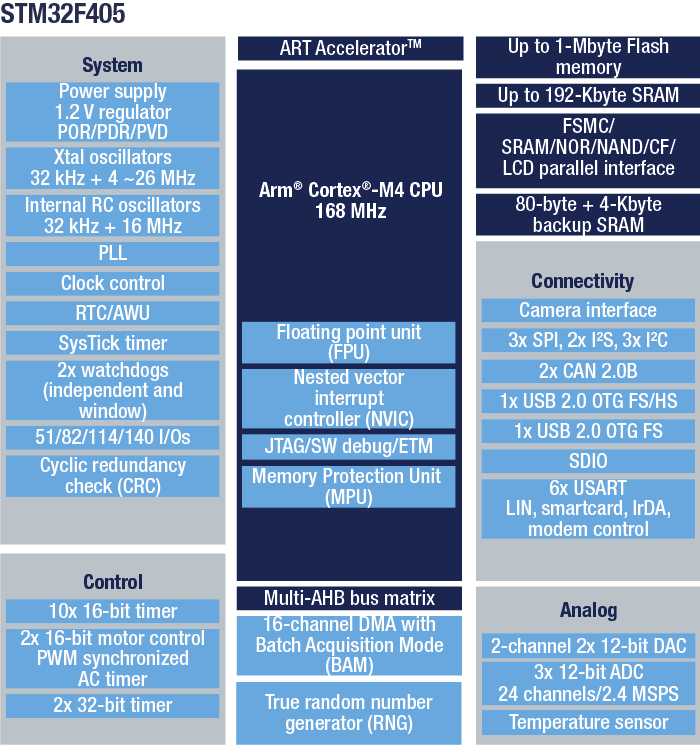
\includegraphics[width=0.7\textwidth]{obrazky/stm32f405_block_diagram}
    \caption{The block diagram of the STM32F405RG MCU~\cite{stm32f405}.}
    \label{fig:stm32f405_block_diagram}
\end{figure}

This MCU confirms to all of the requirement and has enough peripherals to support future development.

% Stepper Driver selection
\subsubsection{Stepper driver}
\label{subsubsec:stepper_driver}
As per the requirements \textbf{C-01} and \textbf{C-02}, the stepper driver shall be able to drive stepper motors with current of up to 2A and feature silent operation.
We decided to use the stepper motor driver ICs developed by Trinamic.
These drivers are nowadays being used for motion control of 3D printers~\cite{prusa_trinamic} and allow for silent operation with their StealthChop technology.
When selecting the driver ICs there were different priorities in mind - first the package should be solderable by hand, secondly with the first revision of the SM4 stepper motor controller we aimed for the ability to power the drivers via a 10-cell Li-Ion power pack, which required maximal input voltage of more than 42 Volts.
The first hardware revision features the TMC2100-TA driver IC, whose main features are shown in the Table~\ref{tab:tmc2100_param}.

\begin{table}[H]
    \centering
    \begin{tabular}{ |p{5cm}|p{7cm}| }
        \hline
        Parameter & Value \\
        \hline
        \hline
        Motor supply voltage & 5-46 V \\
        \hline
        Microsteps & up to 256 \\
        \hline
        Control interface & Step/Dir \\
        \hline
        Configuration interface & GPIO \\
        \hline
        Phase current (RMS) & 1.4 A \\
        \hline
        Advanced stepper control technologies & MicroPlyer, SpreadCycle, StealthChop \\
        \hline
        Package & eTQFP48 \\
        \hline
    \end{tabular}
    \caption{Main parameters of the Trinamic TMC2100-TA driver IC\cite{tmc_2100}.}
    \label{tab:tmc2100_param}
\end{table}


With the second hardware revision, the priorities have shifted and higher phase current was required (\textbf{C-01}) even at the expense of the supply voltage.
The second hardware revision features the TMC2226-SA driver IC, whose properties are shown in the Table~\ref{tab:tmc2226_param}.

\begin{table}[H]
    \centering
    \begin{tabular}{ |p{5cm}|p{7cm}| }
        \hline
        Parameter & Value \\
        \hline
        \hline
        Motor supply voltage & 4.75-29 V \\
        \hline
        Microsteps & up to 256 \\
        \hline
        Control interface & Step/Dir or UART \\
        \hline
        Configuration interface & UART \\
        \hline
        Phase current (RMS) & 2.0 A \\
        \hline
        Advanced stepper control technologies & MicroPlyer, CoolStep, SpreadCycle, StealthChop2, StallGuard4 \\
        \hline
        Package & HTSSOP28 \\
        \hline
    \end{tabular}
    \caption{Main parameters of the Trinamic TMC2226-SA driver IC\cite{tmc_2226}.}
    \label{tab:tmc2226_param}
\end{table}

% TODO describe motion control technologies from Trinamic

\subsubsection{SM4 stepper driver power design}
\label{subsubsec:power_design}

\subsubsection{PCB Design}
\label{subsubsec:pcb_design}
In order for this project to serve as a testbed for new manufacturing technologies, the PCB (Printed Circuit Board) was designed as 4-layer.
The ability to design the board as a 4-layer one was enabled by the 4-layer PCB manufacturing price decrease by China-based PCB manufacturing companies.
Big advantage of designing the PCB as 4-layer one was speedup of hardware development - the 4-layer stackup can be utilized so that there is no need to route power to the ICs.
In our case we chose the inner layers to be filled with copper planes - one connected to GND and the other one connected to +3.3V.
This way whenever a connection to +3.3V or GND was required, simply connecting the pad to new via close-by was sufficient.
Apart from being used for power distribution, the large copper planes allow for better PCB cooling and also for some minor signal connections in cases routing using the outer layers would prove difficult.
The used stackup can be seen in the Figure~\ref{fig:stackup}.

\begin{figure}[H]
    \centering
    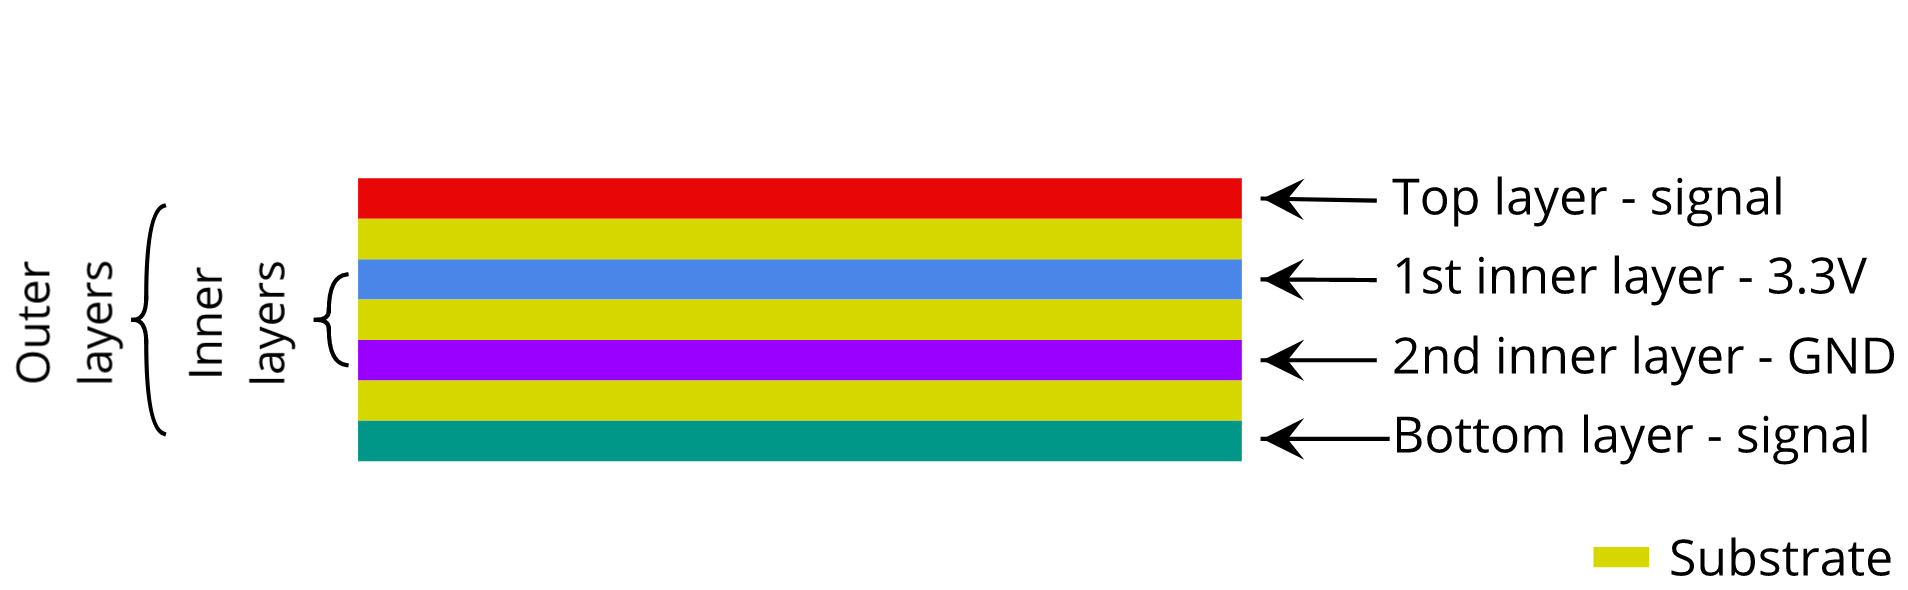
\includegraphics[width=0.9\textwidth]{obrazky/stackup}
    \caption{The 4-layer PCB stackup.}
    \label{fig:stackup}
\end{figure}

Another way to test manufacturing capabilities was utilizing the automated assembly service provided by the China-based PCB manufacturers.
This not-only saved a lot of time with manual assembly, but also enabled us to use smaller components than before - the imperial size 0402.

As for testing out EDA (Electronic Design Aid) software, the KiCAD EDA was used instead of the well-known Eagle.
The KiCAD EDA has improved dramatically in the past years (version 5 and soon to be released version 6), making it great competitor to conventional EDA suites.
The big advantage of KiCAD is a large footprint and symbol library, which often contains even the 3D models and KiCAD itself is able to seamlessly integrate them and render a 3D view of the designed PCB.


\subsection{The MCU and its Auxiliary Circuits}
\label{subsec:mcu_design}

\begin{figure}[H]
    \centering
    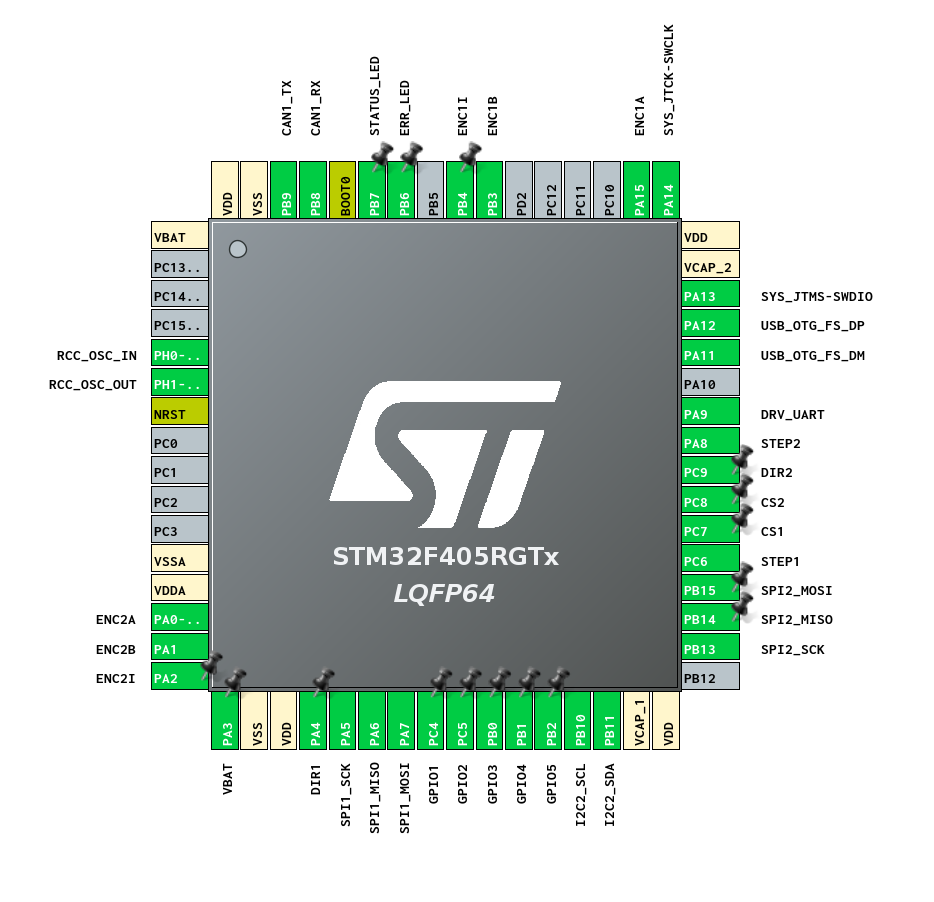
\includegraphics[width=0.9\textwidth]{obrazky/cube_mx}
    \caption{Designing the MCU connections using STM32CubeMX.}
    \label{fig:cubemx}
\end{figure}

\begin{figure}[H]
    \centering
    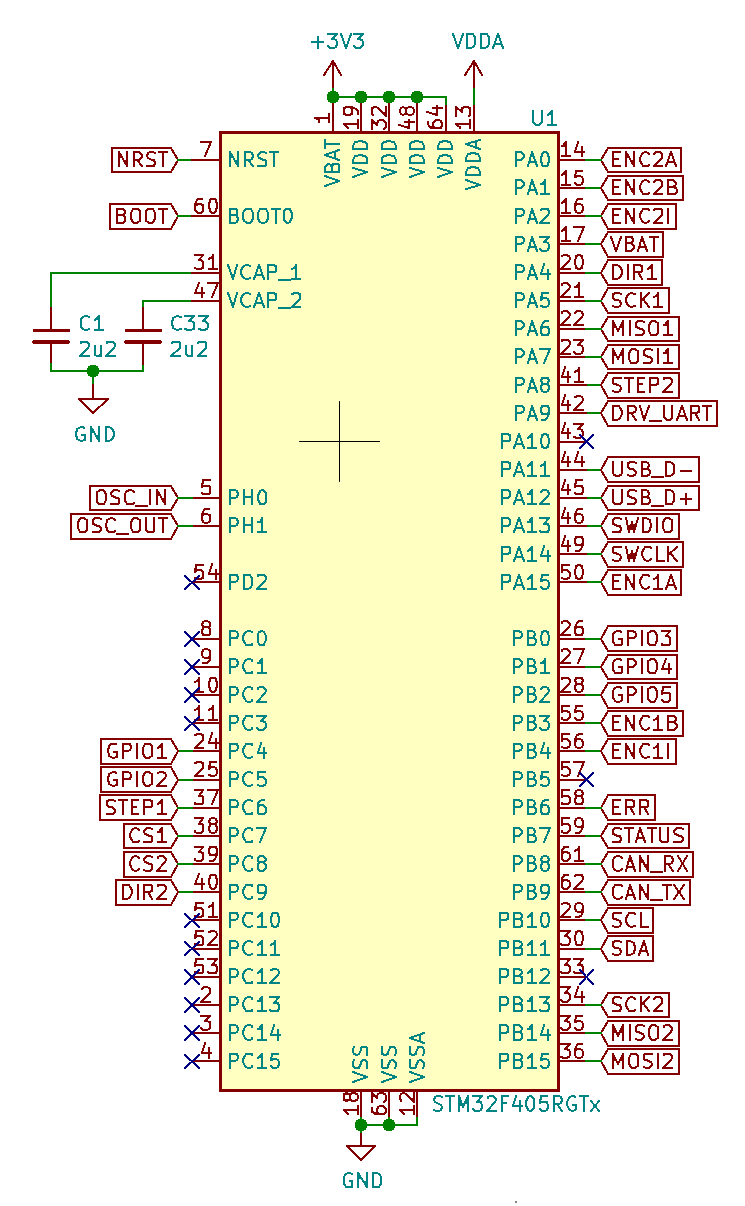
\includegraphics[width=0.6\textwidth]{obrazky/schem_mcu}
    \caption{Designing the MCU connections using STM32CubeMX.}
    \label{fig:schem_mcu}
\end{figure}

\begin{figure}[H]
    \centering
    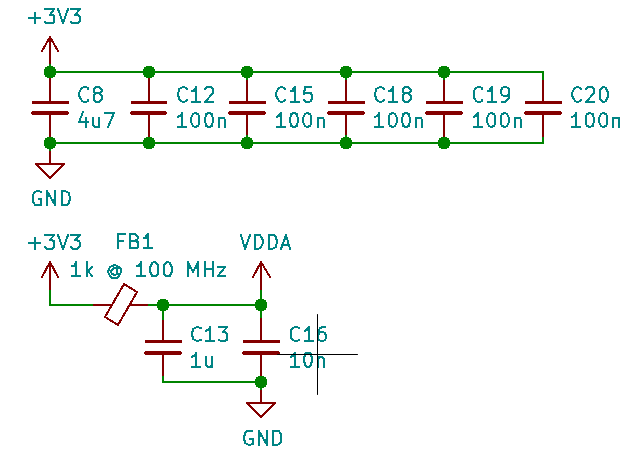
\includegraphics[width=0.6\textwidth]{obrazky/schem_mcu_power_filter}
    \caption{Designing the MCU connections using STM32CubeMX.}
    \label{fig:schem_mcu_power}
\end{figure}


\begin{figure}[H]
    \centering
    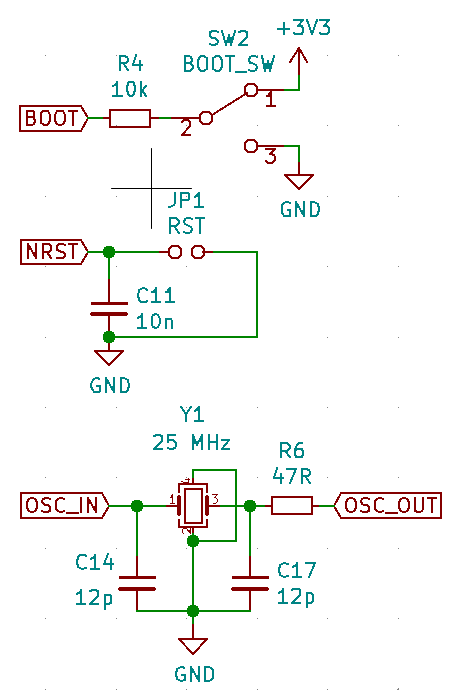
\includegraphics[width=0.4\textwidth]{obrazky/schem_mcu_aux}
    \caption{Designing the MCU connections using STM32CubeMX.}
    \label{fig:schem_mcu_aux}
\end{figure}

\subsection{CAN Bus Circuitry}
\label{subsec:can_circuitry}

\begin{figure}[H]
    \centering
    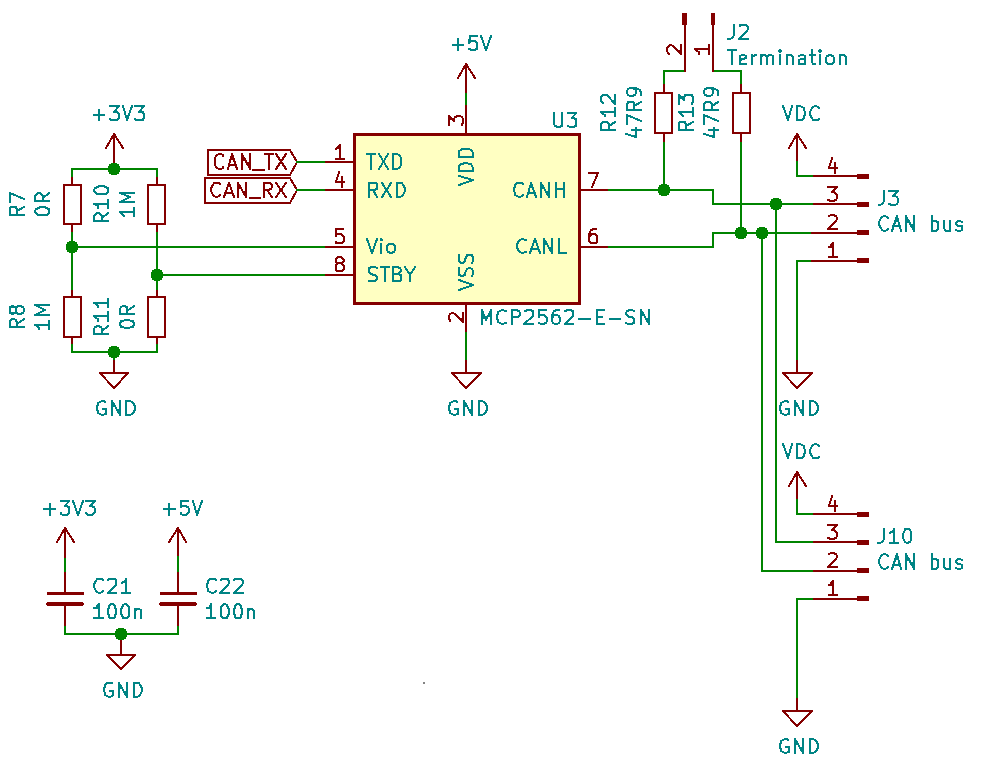
\includegraphics[width=0.9\textwidth]{obrazky/schem_can}
    \caption{Designing the MCU connections using STM32CubeMX.}
    \label{fig:schem_can}
\end{figure}

\subsection{USB Circuitry}
\label{subsec:usb_circuitry}

\begin{figure}[H]
    \centering
    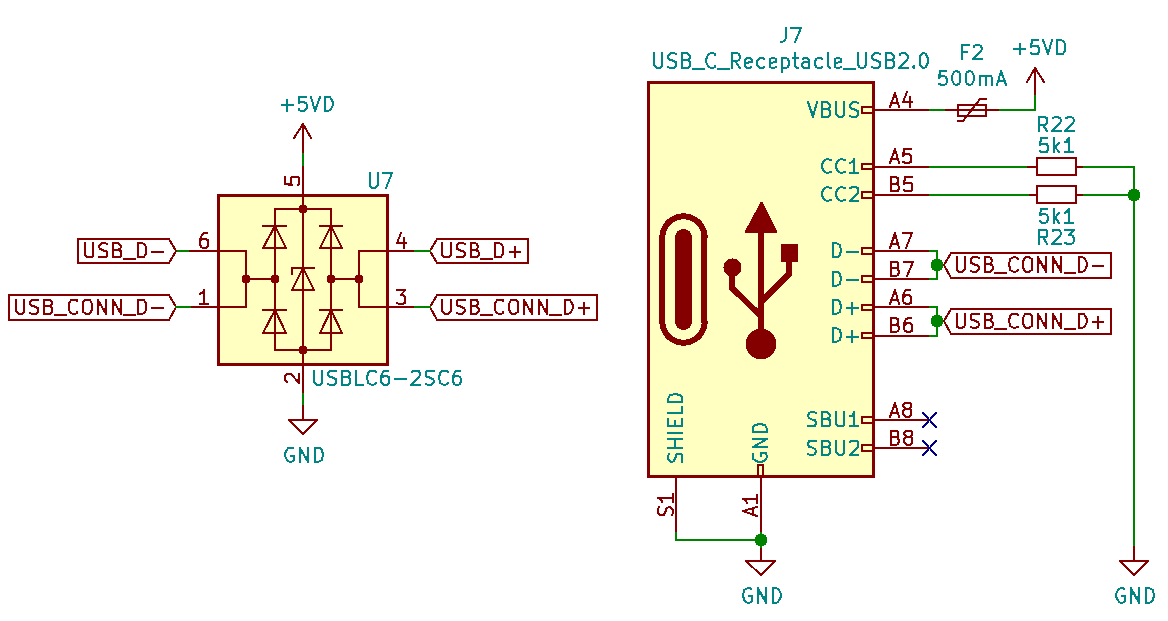
\includegraphics[width=0.9\textwidth]{obrazky/schem_usb}
    \caption{Designing the MCU connections using STM32CubeMX.}
    \label{fig:schem_usb}
\end{figure}

\subsection{Stepper Driver Circuitry}
\label{subsec:stepper_circuitry}

\subsubsection{Revision 1}
\subsubsection{Revision 2}

\begin{figure}[H]
    \centering
    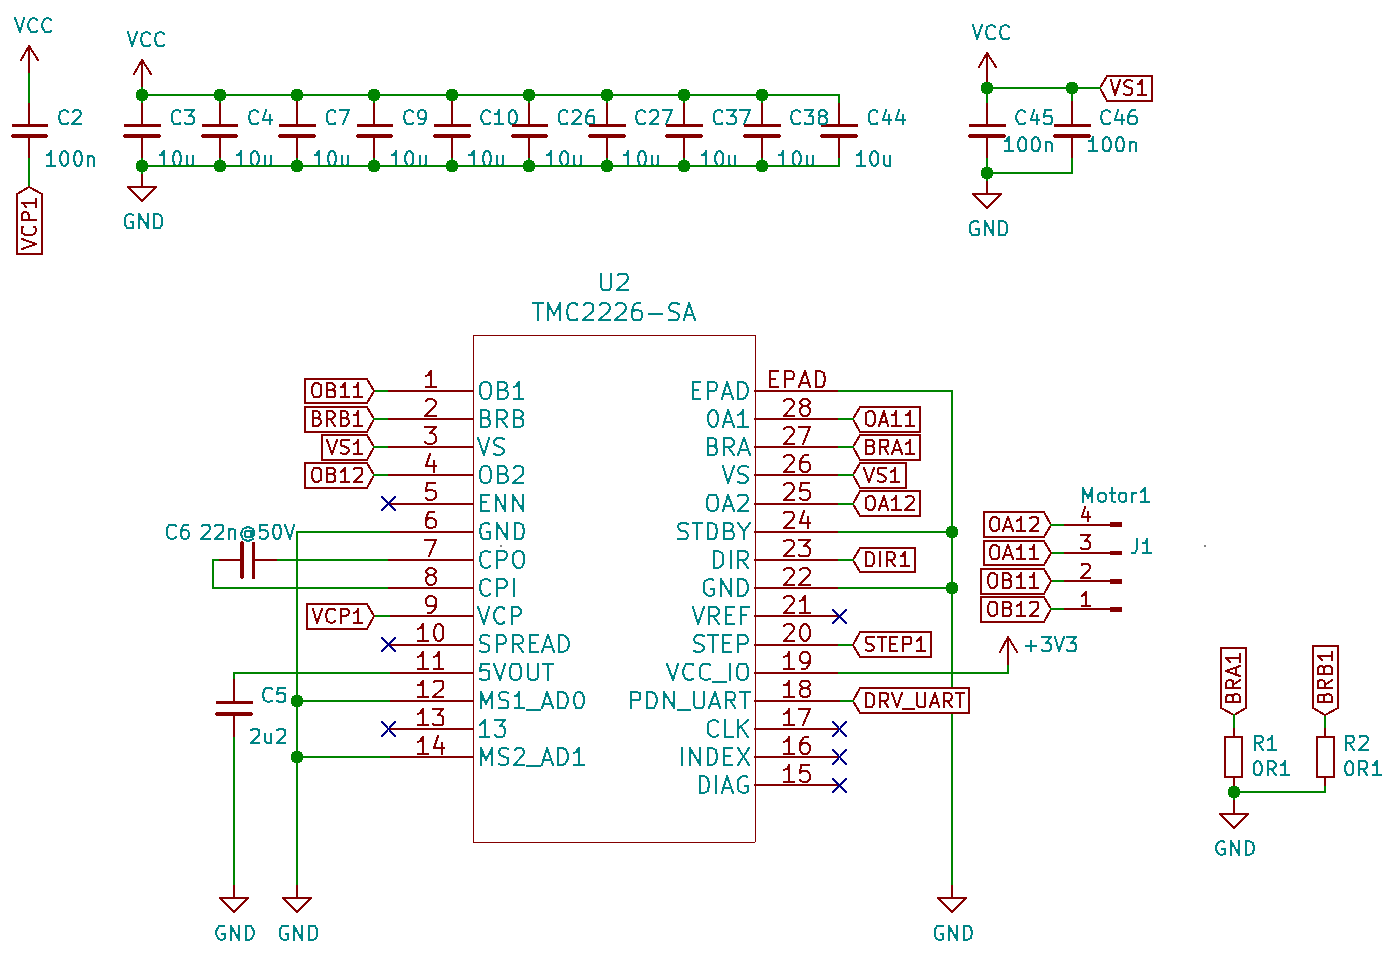
\includegraphics[width=\textwidth]{obrazky/schem_driver_rev2}
    \caption{Designing the MCU connections using STM32CubeMX.}
    \label{fig:schem_driver}
\end{figure}

\subsection{Auxiliary Circuitry and Connectors}
\label{subsec:aux_connectors}

\begin{figure}[H]
    \centering
    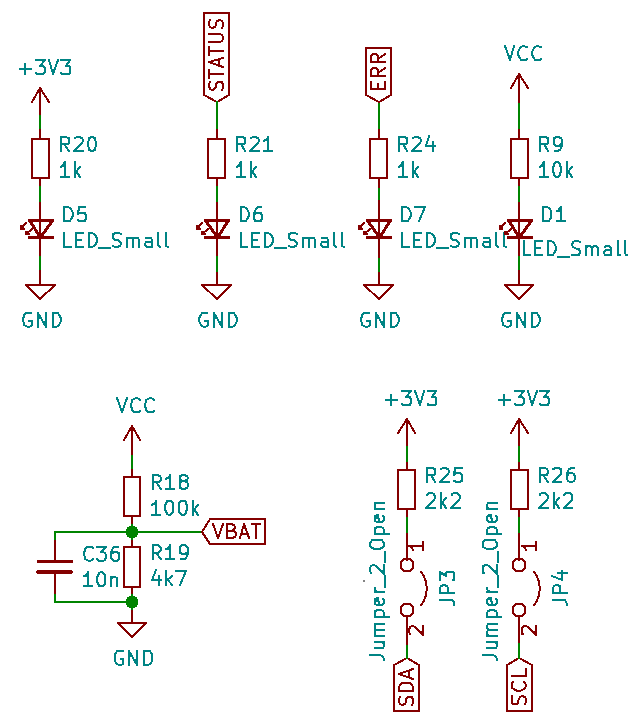
\includegraphics[width=0.6\textwidth]{obrazky/schem_aux}
    \caption{Designing the MCU connections using STM32CubeMX.}
    \label{fig:schem_aux}
\end{figure}


\begin{figure}[H]
    \centering
    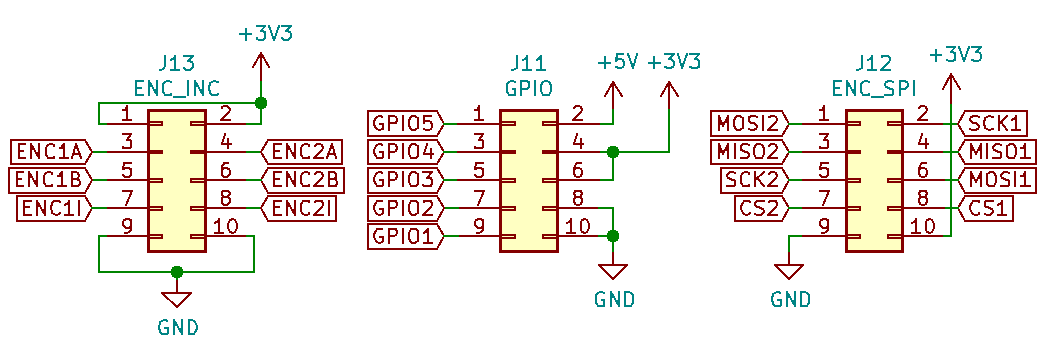
\includegraphics[width=0.9\textwidth]{obrazky/schem_enc_gpio}
    \caption{Designing the MCU connections using STM32CubeMX.}
    \label{fig:schem_enc_gpio}
\end{figure}
% leds, conns, voltage divider

\subsection{PCB Design}
\label{subsec:pcb_design}

\subsection{Manufacturing}
\label{subsec:manufacturing}


\subsection{PCB manufacturing using JLCPCB and KiCAD}
\label{subsec:pcb_manu}
\section{Development of the Bare-Metal Firmware}
\label{sec:firmware}
This Section describes the development of the bare-metal firmware.
First, we go over the firmware architecture, where we describe the technology stack and the architecture itself.
Second, we go over some components of the firmware that are either crucial to the firmware, or their implementation stands out in any way.

\subsection{Firmware Architecture}
\label{subsec:firmware-arch}
Firmware architecture can be described in many ways, we decided to show three ways in which we describe this firmware.
First, we describe the technology stack, describing what crates and libraries we built the hardware upon.
These libraries have mostly been described in the Section~\ref{sec:embedded_rust}.
The technology stack can be seen in the Figure~\ref{fig:firmware_tech_stack}.
When we go from the bottom, to the top, we can see that we access the hardware \acs{mcu} via two crates - the \textbf{stm32-rs} used to access peripheral circuits of the \acs{mcu} and the \textbf{cortex-m} crate used to access the \acs{arm} core of the \acs{mcu}.
The \textbf{stm32f4xx-hal} builds upon the \textbf{stm32-rs} crate and provides Hardware Abstraction Layer over the STM32F4 family and implements the \textbf{embedded-hal} traits.
The \textbf{cortex-m} crate is then used by the RTIC scheduler (described in the Section~\ref{subsec:mut_shared_state}).
As can be seen in the Figure, the firmware itself then builds upon all of these technologies - it accesses the HAL as some peripherals have their abstractions developed, for some special configurations the direct peripheral register access via \textbf{stm32-rs} is used, the RTIC scheduler is used for orchestrating the firmware and for some low-level assembly instructions the \textbf{cortex-m} crate for low level \acs{arm} core access is used.

\begin{figure}[H]
    \centering
    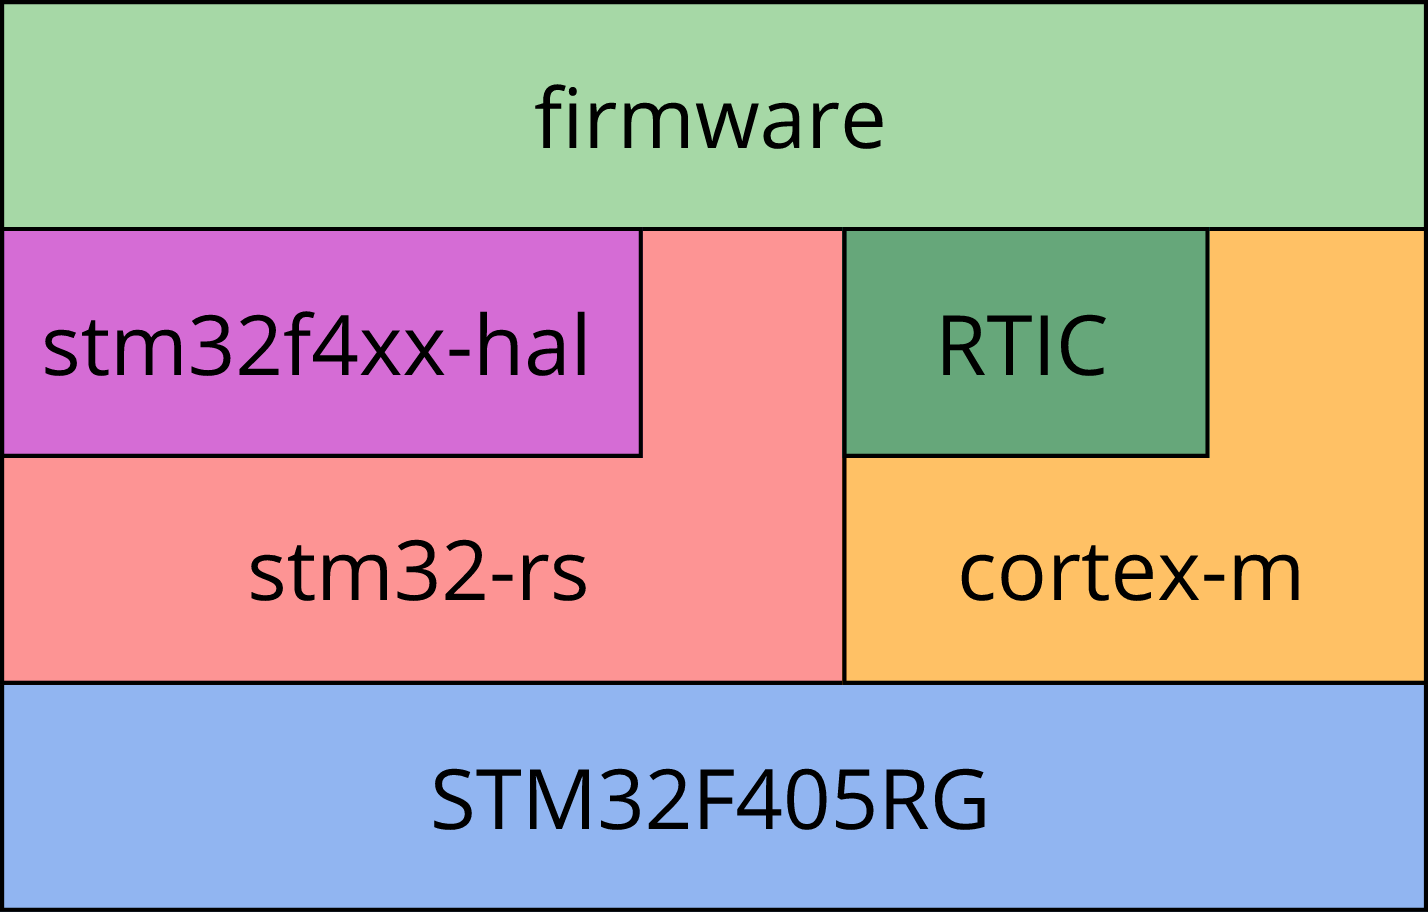
\includegraphics[width=0.5\textwidth]{obrazky/tech_stack}
    \caption{Bare-Metal firmware technology stack.}
    \label{fig:firmware_tech_stack}
\end{figure}

While the technology stack gives us vital information about the architecture, the architecture itself is much more complex and in theory could and should be independent on the used technologies\cite{thomas_pragmatic_2019}.
The architecture overview diagram can be seen in the Figure~\ref{fig:firmware_arch}.
The central part of the architecture is the Object Dictionary (described in Section~\ref{subsec:object_dictionary} and~\ref{subsec:object_dict_impl} (implementation-wise)).
The object dictionary contains the state of the stepper motor controller alongside with configuration.
Part of the object dictionary is also a persistent storage where its values are retained between reboots.
In the center of the firmware, there is also general state that stores variables outside the scope of the Object Dictionary and software failsafe mechanisms, that can manipulate bot the state and object dictionary.
When we look lower in the diagram, we can see that there are the communication interfaces that receive data from and send them to the outer world, usually to some high-level system.
On the other hand, when we look higher in the diagram, that's where the motion control systems operate, they get their data from the object dictionary (control values) and encoders and use these data for controlling the stepper motor driver \acs{ic}s.
The encoders and motor drivers are again connected to the outer world - meaning that they interact with it via the connected motors.

\begin{figure}[H]
    \centering
    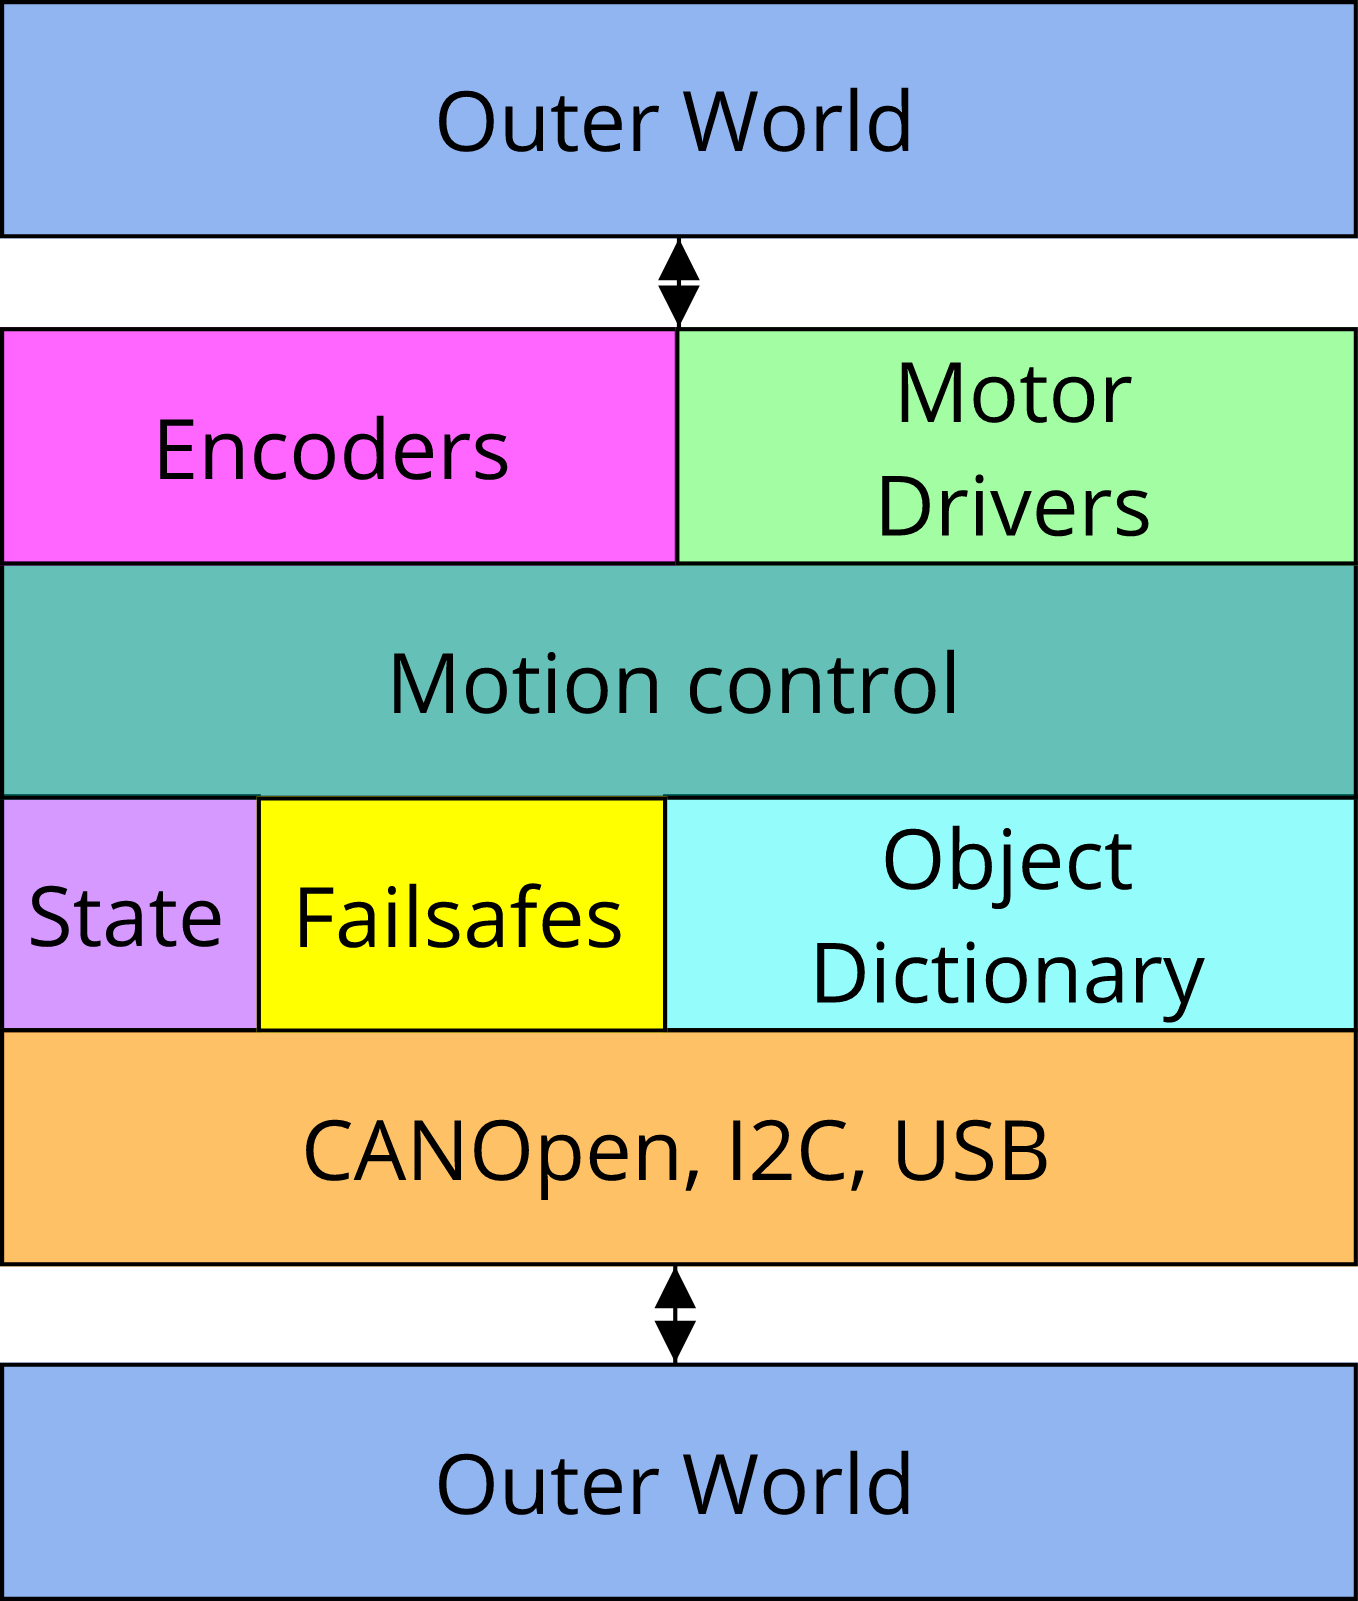
\includegraphics[width=0.5\textwidth]{obrazky/firmware_arch}
    \caption{Bare-Metal firmware architecture.}
    \label{fig:firmware_arch}
\end{figure}

There is one more final point of view on the architecture, which is connected with the project structure.
Given there are two projects - the bare-metal firmware, and the further-described control application, there is a need to share code between those two projects, e.g. share communication models.
An important distinction being, that the bare-metal firmware is also cross-compiled and cross-compiled in a \textbf{no\_std} environment.
Code sharing was solved by creating another project, that is \textbf{no\_std} and is simply called \textbf{shared}, both of the application projects statically link against it.
This can be seen in a diagram presented in the Figure~\ref{fig:component_arch}.
The project structure was adopted from\cite{aparicio_testing_nodate}, which proposes a project structure, that promotes code sharing and testability of all components.

\begin{figure}[H]
    \centering
    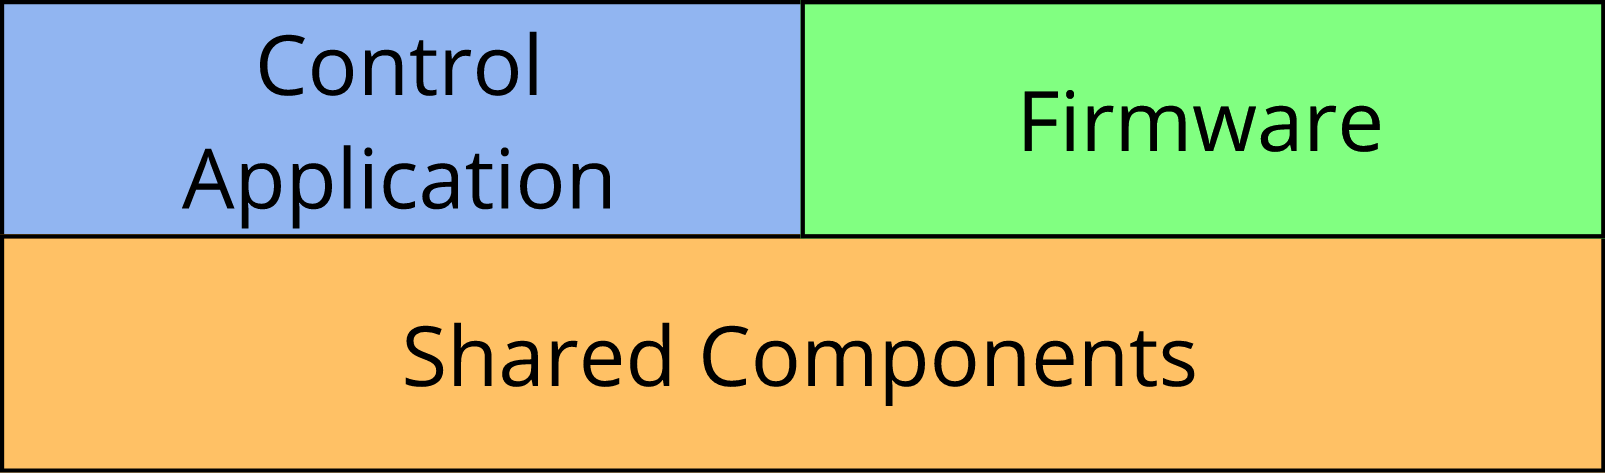
\includegraphics[width=0.5\textwidth]{obrazky/components}
    \caption{Component sharing between the bare-metal firmware and the Control Application.}
    \label{fig:component_arch}
\end{figure}

\subsection{Object Dictionary}
\label{subsec:object_dict_impl}
The importance and role of the Object Dictionary was described in the Sections~\ref{subsec:object_dictionary} and~\ref{subsec:firmware-arch}.
When designing the Object Dictionary, we wanted to design it so that it could be universally used and implemented in multiple ways (e.g. with persistent storage or without one).
The abstraction was done using traits.
The most important trait is the ObjectDictionary trait displayed in the Listing~\ref{lst:od_trait}.
This trait describes the Object Dictionary as a type, that contains information about battery voltage, temperature and an arbitrary number of axes.
The axis is also represented as a trait with accessor methods for specific axis settings (controller settings, current settings, etc.).

\begin{lstlisting}[caption={Trait for abstracting away the Object Dictionary.},label=lst:od_trait]
/// Trait for Object Dictionary abstraction
pub trait ObjectDictionary<const RESOLUTION: u32> {
    /// Returns battery voltage stored in the Object Dictionary.
    fn battery_voltage(&self) -> f32;
    /// Returns temperature stored in the Object Dictionary.
    fn temperature(&self) -> f32;
    /// Sets the battery voltage value in the Object Dictionary.
    fn set_battery_voltage(&mut self, battery_voltage: f32);
    /// Sets the temperature value in the Object Dictionary.
    fn set_temperature(&mut self, temperature: f32);
    /// Returns the configuration of a specific axis.
    fn axis(&self, axis: Axis) -> &dyn AxisDictionary<RESOLUTION>;
    /// Returns a mutable reference the configuration of a specific axis.
    /// This is the only way an axis configuration can be changed
    fn axis_mut(&mut self, axis: Axis) -> &mut dyn AxisDictionary<RESOLUTION>;
}
\end{lstlisting}

To implement a simple Object Dictionary, implementing these traits would be enough, but since we wanted to create an Object Dictionary whose values can be saved in an arbitrary storage, we needed to create another abstraction for storage.
Such an abstraction can be found in the Listing~\ref{lst:storage_trait}.
As can be seen in the Listing, the trait defines loading and saving values of 32-bit floats and boolean values for an arbitrary type of key, that implements the ObjectDictionaryKey.

\begin{lstlisting}[caption={Trait for abstracting away the Object Dictionary storage.},label=lst:storage_trait]
pub trait ObjectDictionaryStorage {
    fn save_f32<KEY: ObjectDictionaryKey>(&mut self,
        key: KEY, value: f32);
    fn save_bool<KEY: ObjectDictionaryKey>(&mut self,
        key: KEY, value: bool);
    fn load_f32<KEY: ObjectDictionaryKey>(&self,
        key: KEY) -> Option<f32>;
    fn load_bool<KEY: ObjectDictionaryKey>(&self,
        key: KEY) -> Option<bool>;
}
\end{lstlisting}

Using all the aforementioned traits we then developed Object Dictionary implementation called the PersistentStoreObjectDictionary, which is generic over the ObjectDictionaryStorage, meaning, that an arbitrary storage type can be used with it.
Similar to the Object Dictionary traits, we also needed to develop a Persistent Store Object Dictionary for axis data, which is also generic over the Object Dictionary Storage and can be seen in the Listing~\ref{lst:persistent_store_dict}.

\begin{lstlisting}[caption={Object Dictionary for persistently storing axis data.},label=lst:persistent_store_dict]
#[derive(Copy, Clone)]
pub struct PersistentStoreAxisDictionary<
    STORAGE: 'static + ObjectDictionaryStorage,
    const RESOLUTION: u32,
> {
    axis: Axis,
    mode: AxisMode,
    enabled: bool,
    target_velocity: Velocity,
    actual_velocity: Velocity,
    target_position: Position<RESOLUTION>,
    actual_position: Position<RESOLUTION>,
    current: CurrentSettings,
    velocity_controller_settings: ControllerSettings,
    position_controller_settings: ControllerSettings,
    velocity_feedback_control_enabled: bool,
    acceleration: f32,
    storage: &'static Mutex<RefCell<STORAGE>>,
}
impl<STORAGE: 'static + ObjectDictionaryStorage, const RESOLUTION: u32>
    AxisDictionary<{ RESOLUTION }> for PersistentStoreAxisDictionary<STORAGE, RESOLUTION>
{
    fn set_accelerating_current(&mut self, current: f32) {
        self.current.set_accelerating_current(current);
        self.storage.lock().borrow_mut().save_f32(
            Key::key_for_axis(AxisKey::AcceleratingCurrent, self.axis),
            current,
        );
    }
...
}
\end{lstlisting}

An important note is that now when any part of the code needs to access the Object Dictionary, it is done by hiding the real implementation behind dynamic dispatch based on the ObjectDictionary trait.

Since we are expecting that the only way a value can be written into the Object Dictionary is using the accessor methods, we employ buffering to make storage reads more scarce, therefore more making the ObjectDictionary more effective.
This basically means that at the firmware startup, all the values are loaded to \acs{ram} and the storage is not accessed when reading.

\subsection{Persistent storage using EEPROM emulation}
\label{subsec:eeprom}
In the previous Section, we discussed development of storage agnostic persistent Object Dictionary and in this section, the way we actually implemented the persistent storage is described.
Persistent storage on MCUs is generally solved by using non-volatile memory that can be either part of the MCU or an external component.
Different memory technologies may be used for both types of the storage.
In general, \acs{fram} (\acl{fram}), \acs{eeprom} (\acl{eeprom}), or flash memories are used.

In order to save space on the \acs{pcb}, save cost, and better utilize the MCU resources we decided to use the internal flash memory to store the user data apart from the driver firmware.
Even though the flash memory may seem straightforward to use since they are ubiquitous, their low level use is not that simple.
A flash memory is generally divided into sectors, that can be several kilobytes or megabytes large.
These sectors can be electrically erased - which means that every bit in the sector is set to 1.
Depending on the memory a word of a specific size can be programmed, but it is only possible to flip the bits in the word to zero~\cite{mansanet_ecorax_nodate, mansanet_ecorax_nodate-1}.
That means that to write a higher number to the word of the memory, the flash needs to be first erased and then programmed.
This is problematic for two reasons:
\begin{enumerate}
    \item sectors generally have the size of several kilobytes, meaning that when you'd want to update the value in the desired word, the whole sector would have to be read to some other memory, erased and then programmed again with the new, updated value,
    \item there is a limited number of whole sector erases, caused by the limitation of hardware.
\end{enumerate}

Fortunately, this problem can be solved by emulating the EEPROM memory as described in ST Application Note AN3969~\cite{stmicro_an3969_2011}.
The application note leverages two FLASH sectors of the same size, where one of them is marked as the active one and the second one is used when the first sector is full.
The working principle is described in the following paragraphs and can be seen in the Figure~\ref{fig:eeprom_emul}.

In the beginning, both of the sectors are erased and one of them is marked as active.
Data are then written to the first sector into simulated cells.
The cells contain a header (which can be understood as a key or a virtual address) and the data.
When a new write is requested, the data are appended behind the already stored data.
When a data with is read using the virtual address, or a key, the sector is traversed from its end, searching for the first occurrence of the key or address.
The first occurrence is the most recent value of the cell marked by the key.
This way we are able to store the value with a specific identifier (key, virtual address) in the flash multiple times.

When no more cells can be written to the active sector, the second sector is marked active, and the data are transmitted to the second sector, taking only the latest value of an identifier into account.
After the transfer, the first sector is erased.

\begin{figure}[H]
    \centering
    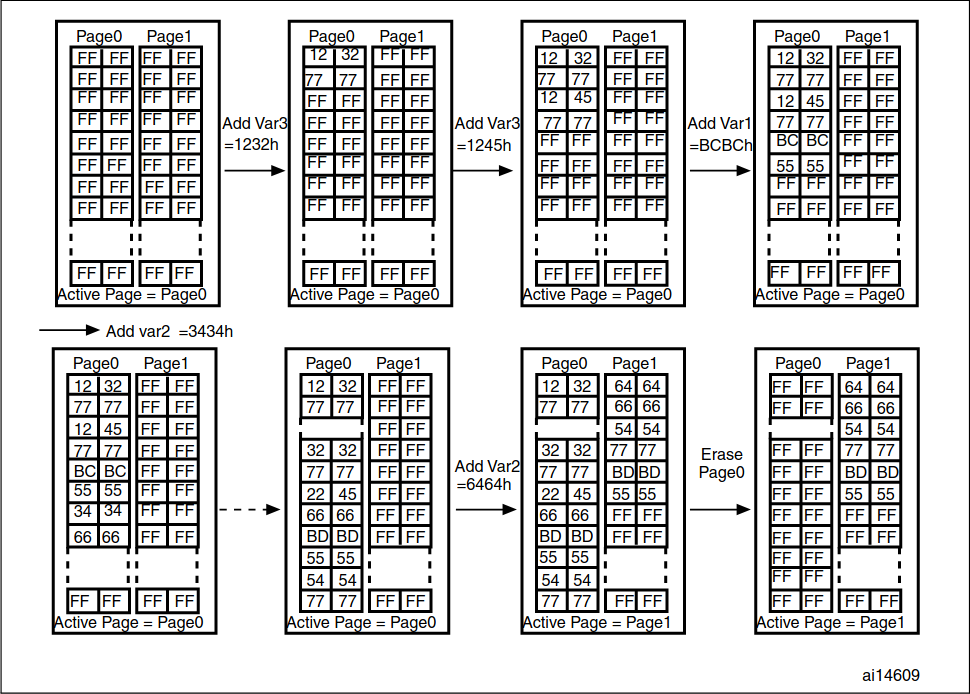
\includegraphics[width=\textwidth]{obrazky/eeprom_emul_principle}
    \caption{EEPROM emulation working principle~\cite{stmicro_an3969_2011}.}
    \label{fig:eeprom_emul}
\end{figure}

Even though the working principle of the EEPROM emulation is simple, there are some technical obstacles in the implementation.
The first obstacle is that the flash memory on the STM32 MCU is split into differently sized sectors, and it is required that the sectors have the same size.
Referring to the Reference Manual~\cite{stmicro_stm32f405rg_nodate} there are a some 16~kilobyte sectors that could be used for the emulation, as can be seen in the Figure~\ref{fig:flash_layout}.
Using the 128~kilobyte sectors would also be possible, but given their size copying values from one sector to another would take too much time and also read access times would be higher.

\begin{figure}[H]
    \centering
    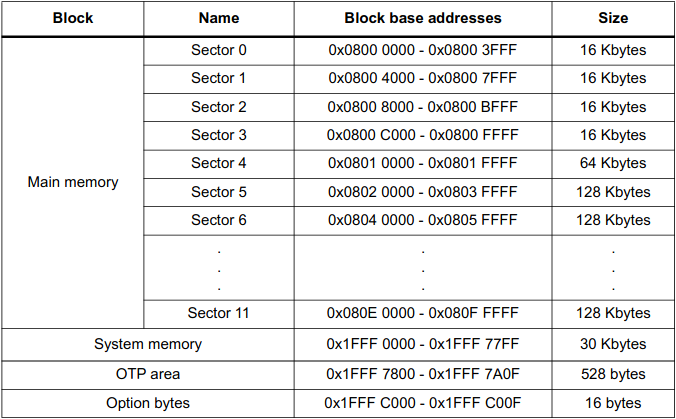
\includegraphics[width=0.8\textwidth]{obrazky/flash_stm}
    \caption{EEPROM emulation working principle~\cite{stmicro_stm32f405rg_nodate}.}
    \label{fig:flash_layout}
\end{figure}

There is however a problem with using the sectors in the beginning of the flash memory as that is where the firmware is usually stored.
The solution to this problem is by leaving the first sector (Sector 0) for the vector table and instructing the linker to place the \textbf{.text} section of the program further in the memory.
According to the documentation of the \textbf{cortex-m} Rust crate~\cite{rust_embedded_devices_wg_rust-embeddedcortex-m_2021}, this can be achieved by adding the line \textbf{\_stext = ORIGIN(FLASH) + OFFSET} to the linker script, where the \textbf{OFFSET} shall be replaced with the offset of the target sector where we want our program to be stored, in our case \textbf{0x0000C000}, which indicates the start of the Sector 3.

As for the actual implementation of the emulation for the STM32F405, we decided to develop our own, as no suitable Rust crate was available for it.
The development was inspired by a crate that implemented the emulation for STM32F103~\cite{dubrov_idubroveeprom_2020} and by following the implementation in the Application Note.
The functions from flash memory access were adopted from an as of the time of writing unmerged Pull Request into the STM32F4 HAL~\cite{astro_implement_2020}.
An example of accessing the emulated persistent storage can be seen in the following Listing~\ref{lst:eeprom}.

\begin{lstlisting}[caption={An example use of the emulated persistent storage.},label=lst:eeprom]
let mut store = Storage::new(device.FLASH);
store
    .init()
    .expect("Failed to initialize emulated storage.");
store.write_f32(0xbeef, 3.14);
let read = store.read_f32(0xbeef).unwrap();
assert_eq!(read, 3.14);
\end{lstlisting}

As can be seen in the Listing~\ref{lst:eeprom}, first we create the object with a parameter of the flash peripheral, then we initialize the emulated storage - this prepares the sectors that are supposed to be used and then we perform a simple write and read operations on the storage.

\subsection{CANOpen Implementation}
\label{subsec:canopen_impl}
The CAN bus on STM32 is implemented in hardware in the bxCAN peripheral.
This peripheral is the same for all of the STM32F \acs{mcu}s, only with slight differences in filter banks and message mailbox sizes.
Given this fact it was possible to develop a crate that supports all of the STM32 \acs{mcu}s, the crate is called \textbf{bxcan} and is developed the stm32-rs organization.

In the past projects described in Chapter~\ref{ch:related_work}, we utilized our own implementation of a driver for the bxCAN peripheral, but since the \textbf{bxcan} crate is well maintained, documented and tested, we decided to discontinue development of the driver and migrate to \textbf{bxcan}.

In order to implement the CANOpen protocols described in the Section~\ref{subsec:canopen}, we developed a simple wrapper over the \textbf{bxcan} crate.
The wrapper is basically a simple proxy that transforms CANOpen protocol data to CAN frames and sends them and parses received CAN frames into CANOpen protocol data.
Upon initialization, the wrapper first configures the bxCAN peripheral, enables interrupts and enables the peripheral itself.

The bxCAN initialization in the wrapper can be seen in the Listing~\ref{lst:canopen_wrapper}.
\begin{lstlisting}[caption={Initializing the bxCAN peripheral in the CANOpen wrapper.},label=lst:canopen_wrapper]
let mut bus = Can::new(bus);
bus.configure(|config| {
    config.set_bit_timing(0x001a000b);
});
bus.enable_interrupts(
    Interrupts::FIFO0_MESSAGE_PENDING | Interrupts::FIFO1_MESSAGE_PENDING,
);
bus.modify_filters()
    .clear()
    .enable_bank(0, Mask32::accept_all());
bus.set_automatic_wakeup(true);
nb::block!(bus.enable()).unwrap();
\end{lstlisting}

When an interrupt handler is invoked, the function \textbf{process\_incoming\_frame} is called, and it returns the type of the CANOpen protocol message, alongside with the received frame.
If the frame contains valid CANOpen message, the CAN frame is further parsed, for example to decode the contents of the PDO as can be seen in the Listing~\ref{lst:can_parse}

\begin{lstlisting}[caption={Initializing the bxCAN peripheral in the CANOpen wrapper.},label=lst:can_parse]
pub fn rx_pdo2<OD, const R: u32>(frame: &Frame, state: &mut DriverState<OD, R>)
where
    OD: ObjectDictionary<R>,
{
    if frame.data().is_none() {
        defmt::warn!("Invalid RxPDO2 received.");
        return;
    }
    if let Ok(pdo) = RxPDO2::try_from(frame.data().unwrap().as_ref()) {
        state
            .object_dictionary()
            .axis_mut(Axis::Axis1)
            .set_target_velocity(Velocity::new(pdo.axis1_velocity));
        state
            .object_dictionary()
            .axis_mut(Axis::Axis2)
            .set_target_velocity(Velocity::new(pdo.axis2_velocity));

        state.invalidate_last_received_speed_command_counter();
    } else {
        defmt::warn!("Malformed RxPDO2 received.");
    }
}
\end{lstlisting}
In the Listing, we can also see accessing the generic ObjectDictionary via the structure \textbf{DriverState}.

\subsection{I\textsuperscript{2}C Slave Implementation}
\label{subsec:i2c_impl}
Implementing I\textsuperscript{2}C slave on a \acs{mcu} is a cumbersome problem, as there is not enough documentation or example code.
Timing of the bus, requiring the slave to react within quite short time makes development and debugging harder, on the other hand with the help of \textbf{defmt} and \acs{rtt} this is not a problem anymore.
We had already developed one implementation of the I\textsuperscript{2}C Slave handling for STM32F0 \acs{mcu} as a part of the KM3 firmware described in the Section~\ref{sec:km3}.
Unfortunately, the STM32F4 family has a different version of the I\textsuperscript{2}C peripheral than the STM32F0, resulting with significant changes to the peripheral handling code, even though the external \acs{api} remained the same.
The I\textsuperscript{2}C2 peripheral is utilized, and it is configured to use the 7 bit addressing mode, with enabled clock stretching to give the \acs{mcu} more time to prepare the data for transfer.
Finally, all the interrupt sources are enabled.
The peripheral has two interrupt vectors - one for data related interrupts \textbf{I2C2\_EV} and one for error related interrupts \textbf{I2C2\_ER}.
When the error related interrupt handler is invoked, the error flags are cleared, and the transfer is reset.
In the data related interrupt handler, the state machine implementing the I\textsuperscript{2}C slave register based protocol (described in the Section~\ref{subsec:i2c}) is implemented.
The result of calling the data interrupt handling function is a state which denotes, what is expected of the higher level system - the data can be either requested or received.
The upper level system then handles transfering the data between the I\textsuperscript{2}C slave implementation's buffers and the Object Dictionary.

% TODO add code describing transfer between I2C and OD

\subsection{USB}
\label{subsec:usb_impl}
The integrated \acs{usb} on the SM4 stepper motor controller has two functions - it enables the possibility to upgrade the firmware via \acs{dfu} (handled by the internal \acs{mcu} bootloader) and provides an interface for configuration (developed by us in the firmware).
For the configuration, the \acs{usb} utilizes the CDC-ACM device class, which means that to the host device, the SM4 controller turns up as a serial port.
Thankfully, given the ubiquity of \acs{usb} devices, crates for implementing \acs{usb} devices on the STM32 are already developed.
There is the crate \textbf{usb-device} providing the \acs{usb} stack and abstractions for hardware\cite{virkkunen_mvirkkunenusb-device_2021}, the \textbf{stm32-usbd}\cite{noauthor_stm32-rsstm32-usbd_2021} implementing the hardware abstraction and \textbf{usbd-serial}\cite{virkkunen_mvirkkunenusbd-serial_2021} implementing the CDC-ACM device class for the \textbf{usb-device} stack.

The implementation of this functionality in the firmware is done via the \textbf{USBProtocol} struct, which is basically a wrapper over the raw USB Serial port functionality.
This wrapper is interrupt driven, quite similarly to the I\textsuperscript{2}C Slave driver, meaning that the received data is parsed when an interrupt handler is invoked, and the data is then exchanged between the wrapper and the Object Dictionary.

An example of configuring the \acs{USB} device can be found in the Listing~\ref{lst:usb}.
\begin{lstlisting}[caption={Initializing the USB device with the CDC-ACM class.},label=lst:usb]
let usb_dev = unsafe {
    UsbDeviceBuilder::new(USB_BUS.as_ref().unwrap(), UsbVidPid(0x16c0, 0x05e1))
        .manufacturer("MH Robotics")
        .product("SM4")
        .serial_number("sm4202101")
        .device_class(usbd_serial::USB_CLASS_CDC)
        .build()
};
\end{lstlisting}
The used device \textbf{VID} and \textbf{PID} were adopted from the VUSB project\cite{noauthor_obdevv-usb_nodate}, that provides them for free with some rules about their use.

\subsection{Stepper control}
\label{subsec:stepper_control}
Movement of stepper motors, controlled using the stepper motor driver \acs{ic}s is generally controlled using the \textbf{STEP/DIR} interface.
This interface consists of two signals, the first of them named~\textbf{STEP} is a square wave signal with variable frequency, where the edges (rising, falling, or both) instruct the driver to move the motor by a microstep.
On the other hand, the second signal named \textbf{DIR} is generally a logic signal, whose logic level denotes the direction of the shaft movement.

Apart from these two digital signals, there is usually an analog signal that is used to set the motor phase current.
In more modern stepper drivers, this analog signal is replaced by a serial digital interface, allowing for finer current setting.

The \textbf{STEP} signal can be generated either in software (by changing the output logical level of a \acs{gpio} pin) or in hardware by utilizing a \acs{pwm} signal with duty cycle of 50 \%.
Both of these approaches have their limitations and advantages.
Generating the signal in software has the advantage of being able to easily count the number of microsteps the motor was commanded to do, on the other hand the upper limit of the maximal frequency is much lower than with hardware generation and this technique uses more computational resources as the signal is generally generated using an interrupt on timer overflow, where the signal logic level needs to be toggled (which requires branching) and the pulse counter needs to be accessed.
Using a timer with \acs{pwm} allows for much higher maximal frequencies, on the other hand counting the pulses can prove to be quite hard.
This issue will be described in more detail in the Section~\ref{subsec:simulated_encoders}.

We decided to utilize the \textbf{STEP} signal generation done by the hardware as we wanted to offload the work from the \acs{mcu} core.

To abstract the real implementation we created a trait (see Section~\ref{subsec:traits}) for setting the microstepping frequency, as can be seen in the Listing~\ref{lst:step_gen_trait}.
Using this trait the software controlling the stepper driver \acs{ic} can use either hardware or software \textbf{STEP} signal generator.

\begin{lstlisting}[caption={Trait for abstracting STEP generation.},label=lst:step_gen_trait]
/// This trait is an abstraction over hardware/software that is capable of generating square wave signal of specific frequency.
/// It is generally implemented by timers.
pub trait StepGenerator {
    /// Sets output frequency of the generator.
    ///
    /// # Arguments
    /// * `frequency` - frequency of the output square wave signal
    fn set_step_frequency(&mut self, frequency: Hertz);
}
\end{lstlisting}

In our case, the trait is implemented by the abstractions over the \acs{mcu}'s advanced control timers 1 and 8.
The abstractions over the timers are based on the timer implementations that can be found in the \textbf{stm32f4xx-hal}, but are preconfigured to generate output \acs{pwm} signals and also to act as a master timer generating clock signal for other timer on compare.

Using this trait, we were able to define a struct which describes the TMC2100 driver as can be seen in the Listing~\ref{lst:tmc2100}.

\begin{lstlisting}[caption={TMC2100 driver.},label=lst:tmc2100]
pub struct TMC2100<G, STEP, DIR, DAC> {
    generator: G,
    _step_pin: STEP,
    dir_pin: DIR,
    current_dac: DAC,
    sense_r: f32,
    microsteps_per_revolution: f32,
}
\end{lstlisting}
In the Listing, we can see, that the driver contains a generic generator, has ownership of the \textbf{STEP} pin (so that no other peripheral can access it), has ownership of the \acs{DIR} pin, \acs{dac} current reference and knows the value of the sense resistor for current setting and microsteps per revolution for \textbf{STEP} output frequency setting.

For a more seamless integration with the motion controller described in the Section~\ref{subsec:motion_control} the trait \textbf{StepperDriver} was declared as can be seen in the Listing~\ref{lst:stepper_driver_trait}.

\begin{lstlisting}[caption={Trait for abstracting the stepper motor driver IC.},label=lst:stepper_driver_trait]
/// This trait is an abstraction over stepper drivers.
/// Generally the drivers have two functions - generate steps and set output current.
pub trait StepperDriver {
    /// Sets output frequency of the driver.
    /// this shall be the angular frequency of the output shaft in revolutions per second.
    ///
    /// # Arguments
    /// * `frequency` - frequency of the output motor shaft in revolutions per second
    fn set_output_frequency(&mut self, frequency: f32);

    /// Sets the target current the driver shall drive the stepper motor with.
    ///
    /// # Arguments
    /// * `current` - the desired current in Amps
    fn set_current(&mut self, current: f32);
}
\end{lstlisting}

This trait was then implemented for the TMC2100 structure, implementing the stepper control itself, as is shown in the Listing~\ref{lst:stepper_driver_impl}.

\begin{lstlisting}[caption={Implementing the StepperDriver trait for TMC2100.},label=lst:stepper_driver_impl]
impl<G, STEP, DIR, DAC> StepperDriver for TMC2100<G, STEP, DIR, DAC>
where
    G: StepGenerator,
    DIR: embedded_hal::digital::v2::OutputPin,
    DAC: DACChannel,
{
    fn set_output_frequency(&mut self, frequency: f32) {
        if frequency < 0.0 {
            self.dir_pin.set_high().ok();
        } else {
            self.dir_pin.set_low().ok();
        };
        self.generator.set_step_frequency(Hertz::new(
            (frequency.abs() * self.microsteps_per_revolution) as u32,
        ))
    }
    fn set_current(&mut self, current: f32) {
        let voltage = (current.abs() * MAX_V_REF as f32 / V_FS * (self.sense_r + R_OFFSET) / 0.707) as u16;
        self.current_dac.set_output_voltage(voltage.min(MAX_V_REF));
    }
}
\end{lstlisting}

\subsection{Simulated encoders}
\label{subsec:simulated_encoders}
The SM4 stepper motor controller is meant to be used without hardware encoder in its default hardware configuration.
This requirement was caused by the reasoning that the motor controller is also targeted for the BPC-PRP course, where students use the distance driven by the wheels to calculate the robot's position in the world's reference frame.
Thankfully, with stepper motor, it is quite easy to simulate encoders by counting the number of microsteps the motor was supposed to move by.
The simulated encoders do not provide real feedback from the system, on the other hand when some conditions are met (no step skipping - no motor overloading), the measurement from them can be quite reliable.

As we already discussed in the Section~\ref{subsec:stepper_control}, we decided to not use counting the microsteps in software, but in hardware instead.
This is done by chaining timers in the \acs{mcu}.
We already mentioned that the timers used to generate \textbf{STEP} signal are configured to be the clock source for other timers, and by counting the clock cycles, we are able to count the number of microsteps the motor was commanded to turn by.

The working principle is really simple and also saves computational power of the \acs{mcu}, but has one disadvantage - the amount of microsteps per sampling period is too low to be used for velocity control, as the difference between the consecutive position reads is usually zero and only sometimes 1.
This poses a big problem for motor control systems of any kind.

Let's have a look at the implementation.
Similarly to what we did with the \textbf{STEP} signal generators, we also declared a trait to abstract away the thing that counts the pulses, so that on the outside it doesn't matter how the counting works.
The trait can be seen in the Listing~\ref{lst:step_counter}.

\begin{lstlisting}[caption={Counter trait for counting STEP pulses.},label=lst:step_counter]
/// Trait used to abstract STEP pulse and other counters.
pub trait Counter {
    /// Return the current internal value of the counter.
    fn get_value(&self) -> u32;
    /// Resets the internal value of the counter.
    fn reset_value(&mut self);
}
\end{lstlisting}
The trait was implemented for the timers 2 and 5 of the \acs{mcu}.

Apart from this trait, an abstraction over the whole encoded was developed.
The abstraction utilizes const generics to define encoder resolution and can be seen in the Listing~\ref{lst:encoder_trait}.

\begin{lstlisting}[caption={Encoder trait for abstracting encoders.},label=lst:encoder_trait]
/// A trait abstracting common encoder functionality.
/// It is suitable for both incremental and absolute encoders.
/// It is designed so its [`Self::sample()`] shall be periodically called with known fixed period,
/// which allows for velocity calculations.
pub trait Encoder<const RESOLUTION: u32> {
    /// Returns the velocity measured by the encoder.
    /// This value is generally calculated from consecutive position readings.
    fn get_velocity(&self) -> Velocity;

    /// Returns the current position of the shaft.
    fn get_position(&self) -> Position<RESOLUTION>;

    /// Sets the sampled position to zero.
    /// This is applicable only with incremental encoders.
    /// Absolute encoders might offset the zero by software.
    fn reset_position(&mut self) -> Position<RESOLUTION>;

    /// This functions shall be periodically called to sample the encoder.
    /// Sampled values are used for position and velocity readings.
    fn sample(&mut self);

    /// This method shall be called with non-directional encoders whenever there is a change of rotation direction.
    /// # Arguments
    /// * `direction` - indicates whether the shaft is now turning in the clockwise or counterclockwise direction.
    fn notify_direction_changed(&mut self, direction: Direction);
}
\end{lstlisting}

Based on this trait and the Counter trait a simulated encoder was developed.
The big advantage being that the the simulated encoder can be easily replaced by another, hardware or software realized encoders.
This Encoder trait is further used in the motion controller.

\subsection{Device Monitoring}
\label{subsec:device_monitoring}
In order to provide status and health information, simple device monitoring is employed.
The monitoring system periodically reads internal \acs{mcu} temperature and the motor voltage.
This functionality is implemented by accessing the internal \acs{mcu} \acs{adc}.
The internal \acs{adc} utilizes the Successive approximation principle and supports up-to 19 channels\cite{stmicro_stm32f405xx_2020}.
The \acs{adc} is configured to read the two channels and to use \acs{dma} to transfer the values from the peripheral to the program's memory.
Both \acs{adc} configuration and \acs{dma} transfer are already implemented in the \textbf{stm32f4xx-hal} crate, meaning that no low-level peripheral access code was required.
The monitoring data are periodically transferred to the Object Dictionary by the higher-level code.

First, we configure the \acs{adc} as can be seen in the Listing~\ref{lst:adc}.
We set the \acs{dma} transfer mode to \textbf{Continuous} (which reissues a \acs{dma} request on every start of conversion) and enable scan mode, which scans all the channels in the sequence.
Further, both of the channels are configured, with assignment to pin/ or special channel, order in the conversion sequence and sample time, which denotes for how many clock cycles the sample-and-hold circuits samples.
Finally, the temperature and VRef channel measurement is enabled as it is not enabled by default by the hardware.

\begin{lstlisting}[caption={Configuring ADC for temperature and voltage monitoring.},label=lst:adc]
let mut adc = Adc::adc1(raw_adc, true, adc_config);
let adc_config = AdcConfig::default()
     .dma(Dma::Continuous)
     .scan(Scan::Enabled);
adc.configure_channel(&Temperature, Sequence::One, SampleTime::Cycles_480);
adc.configure_channel(&battery_voltage, Sequence::Two, SampleTime::Cycles_480);
adc.enable_temperature_and_vref();
\end{lstlisting}

Next, we configure the \acs{dma} transfer, as can be seen in the Listing~\ref{lst:dma}.
We configure the \acs{dma} controller to issue an interrupt when the transfer is complete, to increment addresses only in memory and not in the peripheral and we disable double buffering.

\begin{lstlisting}[caption={Configuration of the DMA controller for ADC transfers.},label=lst:dma]
let first_buffer = singleton!(: [u16; 2] = [0; 2]).unwrap();
let config = DmaConfig::default()
    .transfer_complete_interrupt(true)
    .memory_increment(true)
    .double_buffer(false);
let transfer = Transfer::init(dma, adc, first_buffer, None, config);
\end{lstlisting}

The monitoring system is then periodically asked to poll data from the \acs{adc} by starting the transfer as can be seen in the following Listing~\ref{lst:adc_poll}.
\begin{lstlisting}[caption={Polling the ADC.},label=lst:adc_poll]
self.transfer.start(|adc| {
    adc.start_conversion();
});
\end{lstlisting}
When the \acs{dma} transfer complete interrupt routine is called, the next transfer is prepared and the measured data is processed using factory calibration and formulae that can be found in the reference manual\cite{stmicro_stm32f405xx_2020}.
The final two coefficients in the battery\_voltage calculation represent the voltage divider described in the Section~\ref{subsec:aux_connectors}.
The preparation and calculation is shown in the Listing~\ref{lst:adc_isr}.
\begin{lstlisting}[caption={Processing the data measured by the ADC.},label=lst:adc_isr]
let (buffer, _) = self
    .transfer
    .next_transfer(self.buffer.take().unwrap())
    .unwrap();
let raw_temp = buffer[0];
let raw_volt = buffer[1];
self.buffer = Some(buffer);
let cal30 = VtempCal30::get().read() as f32;
let cal110 = VtempCal110::get().read() as f32;
self.temperature = (110.0 - 30.0) * ((raw_temp as f32) - cal30) / (cal110 - cal30) + 30.0;
self.battery_voltage = (raw_volt as f32) / ((2_i32.pow(12) - 1) as f32) * 3.3 / 4.7 * 104.7;
\end{lstlisting}

\subsection{Motion Control}
\label{subsec:motion_control}
% psd, ramping

\begin{figure}[H]
    \centering
    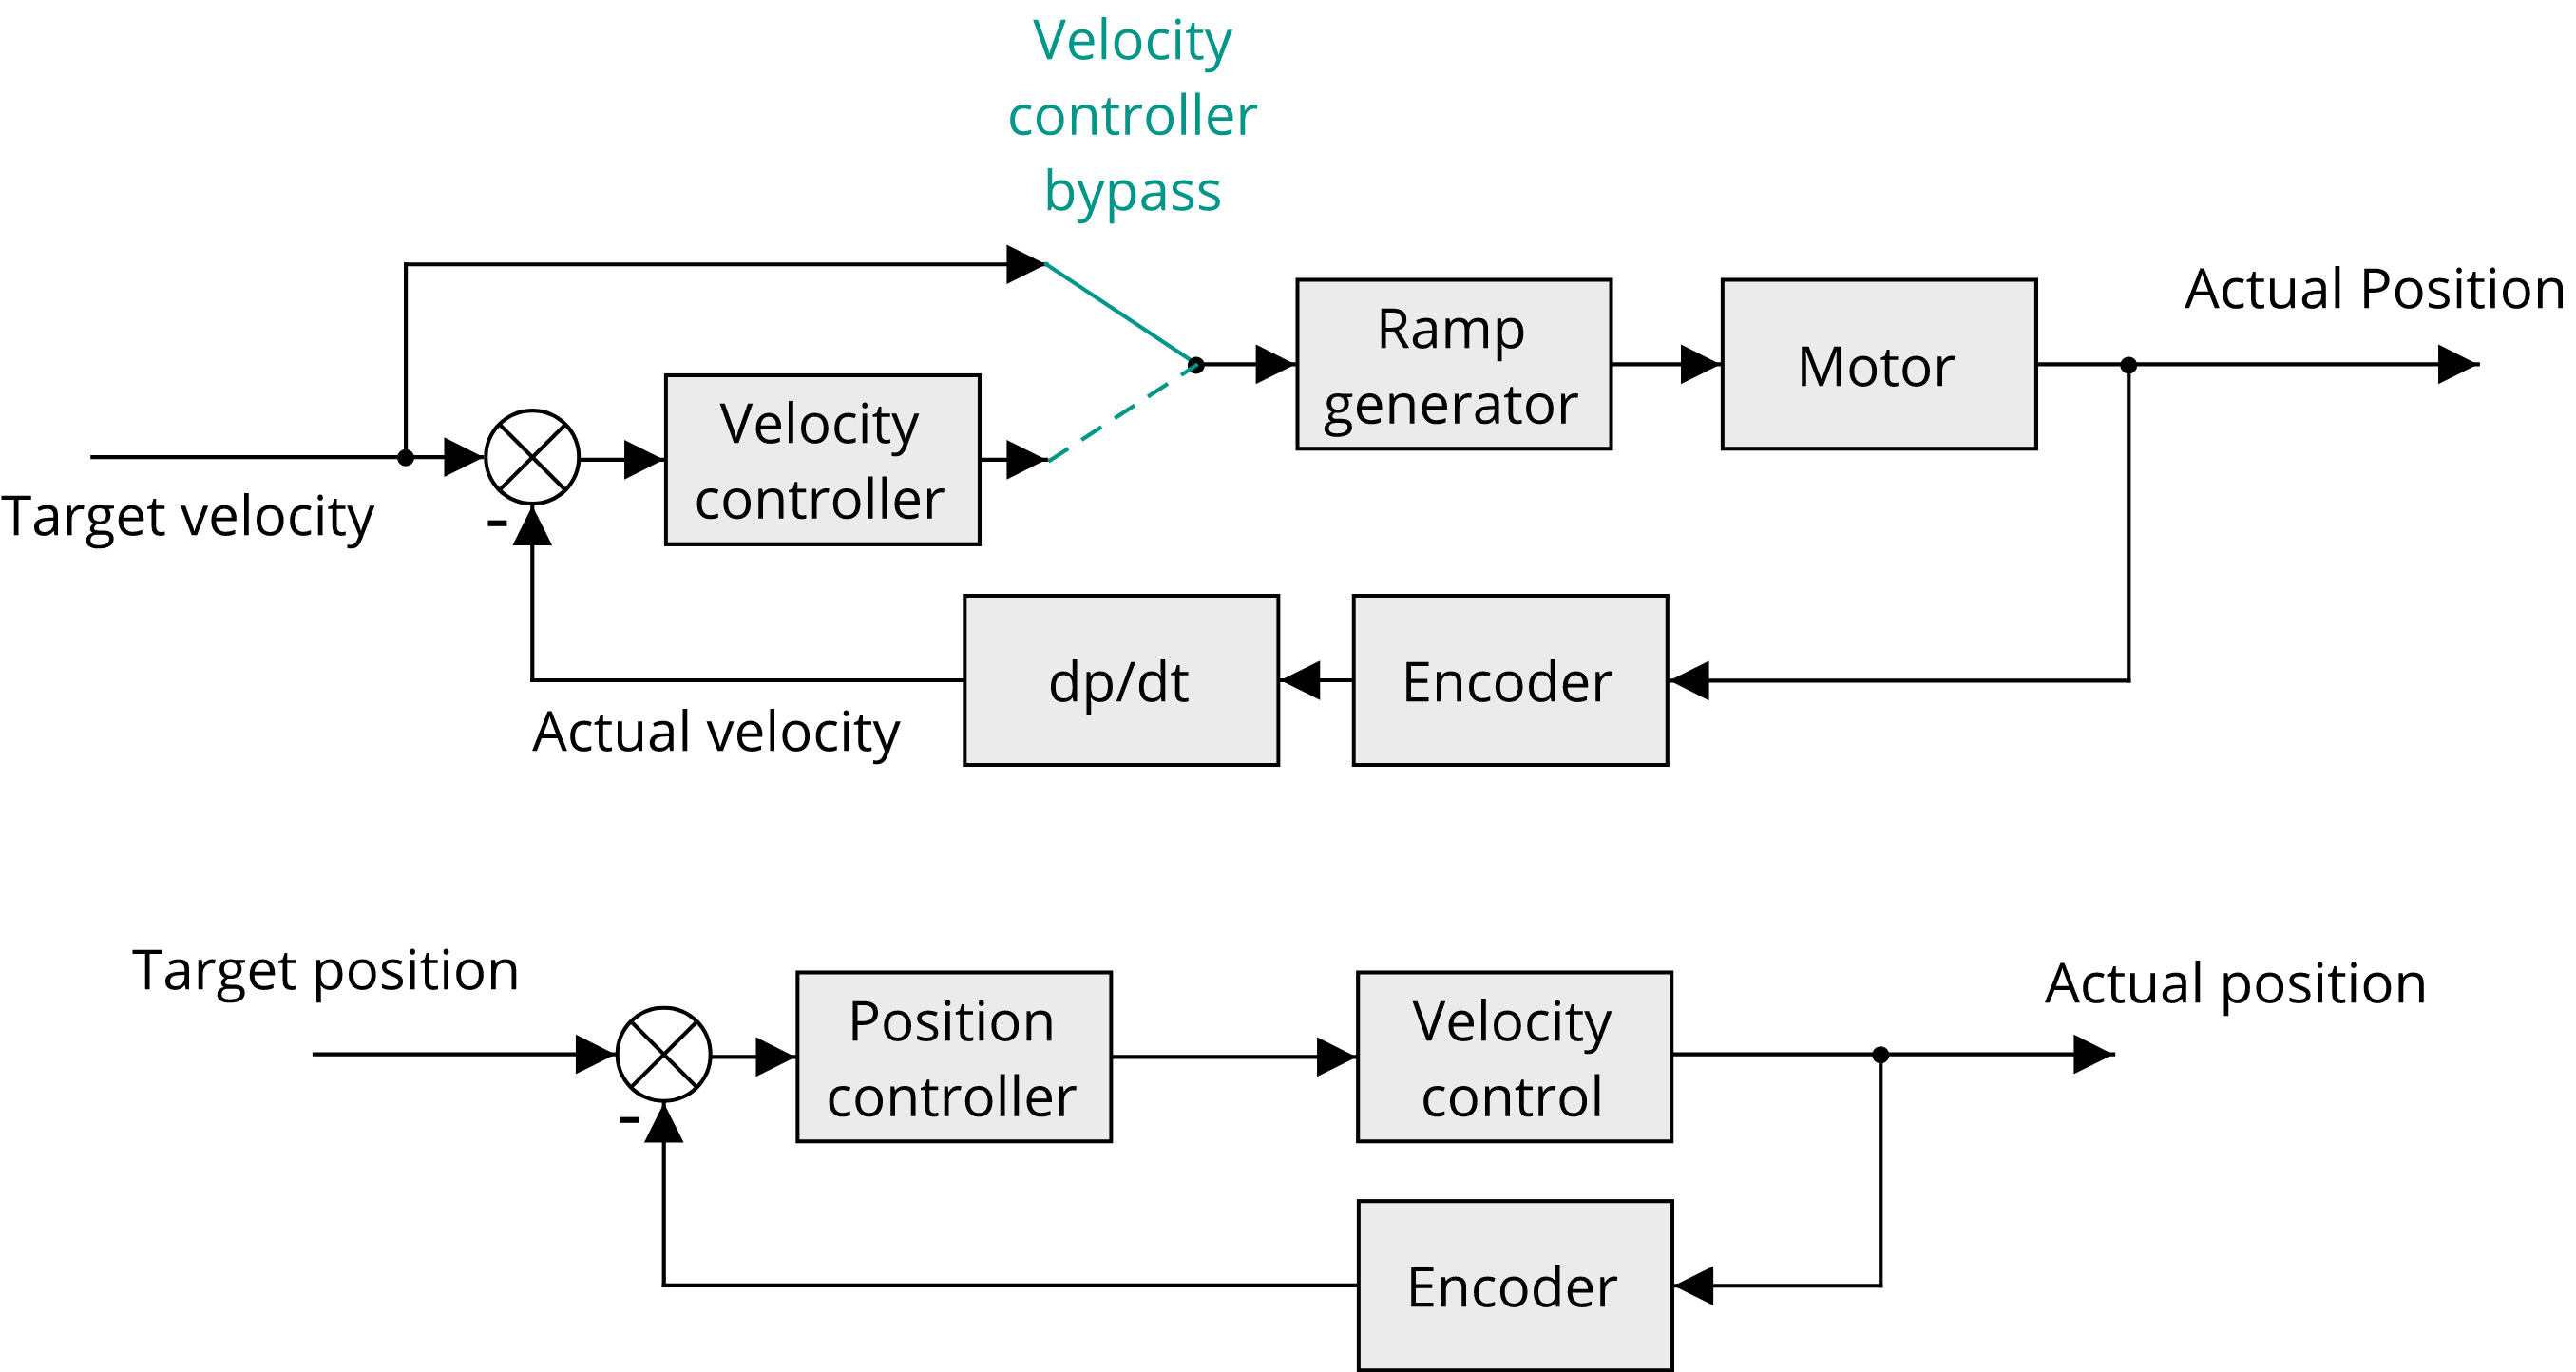
\includegraphics[width=\textwidth]{obrazky/motion_control}
    \caption{Motion control schematic.}
    \label{fig:motion_control}
\end{figure}


\subsection{Persistent storage using EEPROM emulation}
\label{subsec:eeprom}
The SM4 stepper motor controller needs persistent storage to save configuration and data.
Persistent storage on MCUs is generally solved by using non-volatile memory that can be either part of the MCU or an external component.
Different memory technologies may be used for both types of the storage.
In general, FRAM (Ferroelectric Random Access Memory), EEPROM (Electrically Erasable programmable read-only memory), or flash memories are used.

In order to save space on the PCB, save cost, and better utilize the MCU resources we decided to use the internal flash memory to store the user data apart from the driver firmware.
Even though the flash memory may seem straightforward to use since they are ubiquitous, their low level use is not that simple.
A flash memory is generally divided into sectors, that can be several kilobytes or megabytes large.
These sectors can be electrically erased - which means that every bit in the sector is set to 1.
Depending on the memory a word of a specific size can be programmed, but it is only possible to flip the bits in the word to zero~\cite{ecorax_flash}.
That means that to write a higher number to the word of the memory, the flash needs to be first erased and then programmed.
This is problematic for two reasons:
\begin{enumerate}
    \item sectors generally have the size of several kilobytes, meaning that when you'd want to update the value in the desired word, the whole sector would have to be read to some other memory, erased and then programmed again with the new, updated value,
    \item there is a limited number of whole sector erases, caused by the limitation of hardware.
\end{enumerate}

Fortunately, this problem can be solved by emulating the EEPROM memory as described in ST Application Note AN 3969~\cite{eeprom_appnote}.
The application note leverages two flash sectors of the same size, where one of them is marked as the active one and the second one is used when the first sector is full.
The working principle is described in the following paragraphs and can be seen in the Figure~\ref{fig:eeprom_emul}.

In the beginning, both of the sectors are erased and one of them is marked as active.
Data are then written to the first sector into simulated cells.
The cells contain a header (which can be understood as a key or a virtual address) and the data.
When a new write is requested the data are appended behind the already stored data.
When a data with is read using the virtual address or a key, the sector is traversed from its end, searching for the first occurrence of the key or address.
The first occurrence is the most recent value of the cell marked by the key.
This way we are able to store the value with a specific identifier (key, virtual address) in the flash multiple times.

When no more cells can be written to the active sector, the second sector is marked active and the data are transmitted to the second sector, taking only the latest value of an identifier into account.
After the transfer, the first sector is erased.

\begin{figure}[H]
    \centering
    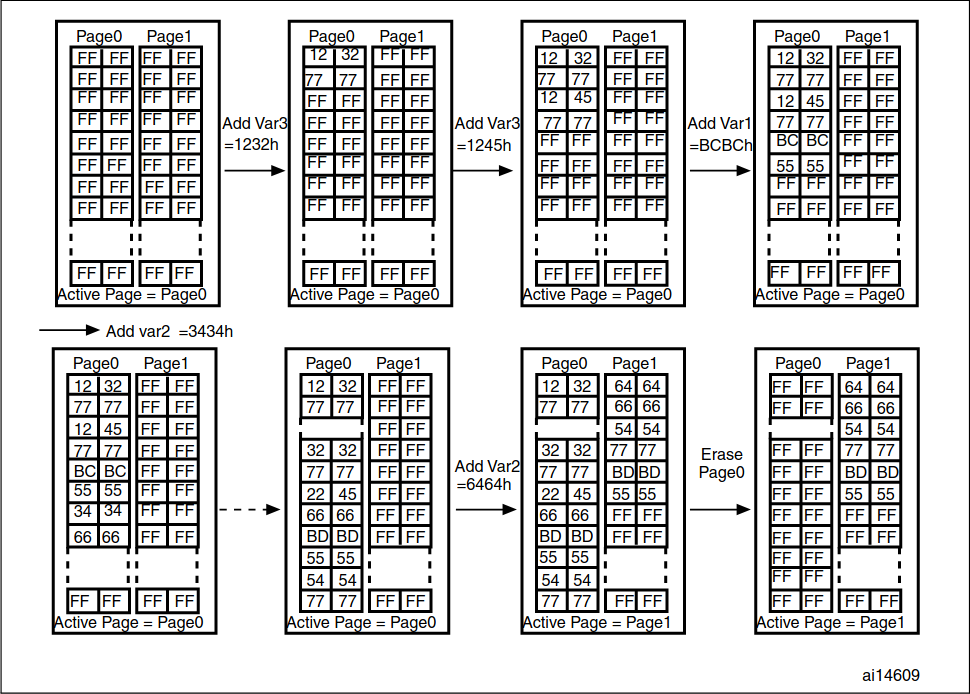
\includegraphics[width=\textwidth]{obrazky/eeprom_emul_principle}
    \caption{EEPROM emulation working principle~\cite{eeprom_appnote}.}
    \label{fig:eeprom_emul}
\end{figure}

Even though the working principle of the EEPROM emulation is simple, there are some technical obstacles in the implementation.
The first obstacle is that the flash memory on the STM32 MCU is split into differently sized sectors and it is required that the sectors have the same size.
Referring to the Reference Manual~\cite{stm32f405_ref_manual} there are a some 16~kilobyte sectors that could be used for the emulation, as can be seen in the Figure~\ref{fig:flash_layout}.
Using the 128~kilobyte sectors would also be possible, but given their size copying values from one sector to another would take too much time and also read access times would be higher.

\begin{figure}[H]
    \centering
    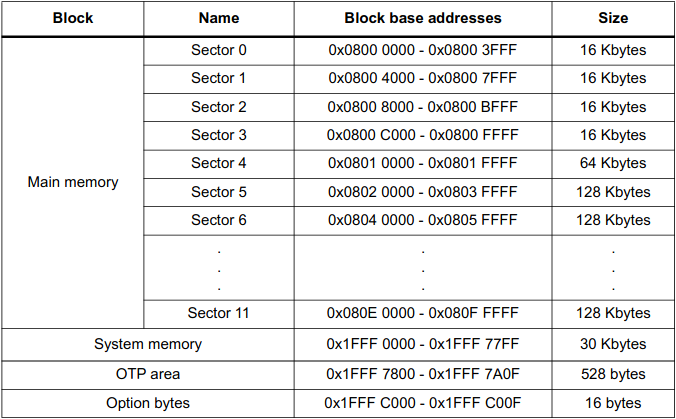
\includegraphics[width=0.8\textwidth]{obrazky/flash_stm}
    \caption{EEPROM emulation working principle~\cite{stm32f405_ref_manual}.}
    \label{fig:flash_layout}
\end{figure}

There is however a problem with using the sectors in the beginning of the flash memory as that is where the firmware is usually stored.
The solution to this problem is by leaving the first sector (Sector 0) for the vector table and instructing the linker to place the \textbf{.text} section of the program further in the memory.
According to the documentation of the \textbf{cortex-m} Rust crate~\cite{crate-cortext-m}, this can be achieved by adding the line \textbf{\_stext = ORIGIN(FLASH) + OFFSET} to the linker script, where the \textbf{OFFSET} shall be replaced with the offset of the target sector where we want our program to be stored, in our case \textbf{0x0000C000}, which indicates the start of the Sector 3.

As for the actual implementation of the emulation for the STM32F405, we decided to develop our own, as no suitable Rust crate was available for it.
The development was inspired by a crate that implemented the emulation for STM32F103~\cite{crate_f103_eeprom} and by following the implementation in the Application Note.
The functions from flash memory access were adopted from an as of the time of writing unmerged Pull Request into the STM32F4 HAL~\cite{pr_flash}.
An example of accessing the emulated persistent storage can be seen in the following Listing~\ref{lst:eeprom}.

\begin{lstlisting}[caption={An example use of the emulated persistent storage.},label=lst:eeprom]
let mut store = Storage::new(device.FLASH);
store
    .init()
    .expect("Failed to initialize emulated storage.");
store.write_f32(0xbeef, 3.14);
let read = store.read_f32(0xbeef).unwrap();
assert_eq!(read, 3.14);
\end{lstlisting}

As can be seen in the Listing~\ref{lst:eeprom}, first we create the object with a parameter of the flash peripheral, then we initialize the emulated storage - this prepares the sectors that are supposed to be used and then we perform a simple write and read operations on the storage.

\section{Development of the control application}


\chapter{Results}

\section{Demonstration \#1 - A simple mobile robot}

\epigraph{
    Any exploration program which "just happens" to include a new launch vehicle is, de facto, a launch vehicle program. \\ \\
    (alternate formulation) The three keys to keeping a new human space program affordable and on schedule: \\
1)  No new launch vehicles. \\
2)  No new launch vehicles. \\
3)  Whatever you do, don't develop any new launch vehicles.}{Akin's Laws of Spacecraft Design\cite{phillip_koopman_better_2010}}

\chapter*{Conclusion, Discussion and Future work}
\phantomsection
\addcontentsline{toc}{chapter}{Conclusion, Discussion and Future work}
In this thesis, we described the development of a dual-channel stepper motor controller we named SM4.
We developed both the hardware and software.
As for the hardware development, we utilized the STM32F405 MCU and Trinamic stepper motor driver ICs as the basis of the design.
As for PCB design, we utilized a 4-layer PCB to decrease the development time, and we utilized the JLCPCB's manufacturing service alongside the PCB assembly service.
Two revisions of the PCB were designed and manufactured, two of each revision PCBs were assembled.
Even though the second revision of the PCB is more advanced than the first one, there is still plenty of room for improvements, which we came across during the development.
The schematic and PCBs were designed in the KiCAD EDA suite, which proved useful, given the fact that KiCAD has a large footprint and symbol library.

As for the development of the software, we utilized the Rust programming language for both the bare-metal firmware and the control application.
Unfortunately, the firmware, as of now, supports only the first revision of the hardware.
Developing the firmware in Rust proved useful, as there is great support for developing on bare-metal, given there is a large community for developing device drivers, HALs, and tooling.
During the development, we utilized many of the language's features, especially when developing abstractions over the hardware where we utilized traits and generics.
We believe that given the developed abstractions the firmware can be easily extended and improved.

We believe that the tooling that currently exists surpasses the tooling available for other languages and ecosystems.
The language's features provide memory and data race safety for embedded systems while not impeding the code size or performance.
Given our experience with developing embedded firmware for this project and several other ones described earlier, we firmly believe that the Rust programming language is the right way forward as it brings features never deemed possible for embedded systems development.

Apart from the firmware, we also developed a simple control application for personal computers that is now capable of only controlling the stepper motor controller but not of configuring it.
The control application is now able to control the controller's axis in both velocity and position modes.

Even though there is still a lot of work to be done, we believe that the controller is currently usable and be deployed, for example, to be part of the BPC-PRP course.

\section{Future work}
\label{sec:fut_job}
We are hoping to continue working on the stepper motor controller in the future.
We would like to greatly extend and improve both the hardware and software (and both the firmware and the control application).
Some of the requirements were not completely fulfilled, and we are aiming to revisit them.
A big part of the future development will be finishing the documentation and automated testing.
Extending the firmware with support for the second hardware revision will be a priority since the new stepper motor controller IC is much more powerful than the one in the first revision.
We are also planning to try integrating real hardware encoders to try out the suitability of the abstractions and the ability to control the motors with proper feedback.
We will also aim for full conformance with the CANOpen standard to allow for seamless integration with other systems.
We are also looking into continuing the development using Rust programming language for embedded systems, either by developing more projects using it or contributing to the existing ecosystem by developing the tooling and libraries.


%\bibliographystyle{unsrturl}
\printbibliography[heading=bibintoc]
%\addcontentsline{toc}{chapter}{Bibliography}
%\bibliography{text/literatura}
%\nocite{*}

\cleardoublepage
\chapter*{\listofabbrevname}
\phantomsection
\addcontentsline{toc}{chapter}{\listofabbrevname}

\begin{acronym}[KolikMista]

	\acro{zkTemp}		% název
		[Šířka levého sloupce Seznamu symbolů a zkratek]								% zkratka
		{je určena šířkou parametru prostředí \texttt{acronym} (viz řádek~1 výpisu zdrojáku na~str.\,\pageref{lst:zkratky})}
											% rozvinutí zkratky

	\acro{zkDummy}
		[KolikMista]
		{pouze ukázka vyhrazeného místa}

	\acro{DSP}		% název/zkratka
		{číslicové zpracování signálů -- Digital Signal Processing}
											% rozvinutí zkratky
	%%% bsymfvz
	\acro{symfvz}						% název
		[\ensuremath{f_\textind{vz}}] % symbol
		{vzorkovací kmitočet}					% popis
	%%% esymfvz

\end{acronym}


\appendix
%%% Vysázení seznamu příloh
% (vynechejte, pokud máte dvě nebo méně příloh)
\listofappendices

%%% Vložení souboru 'text/prilohy' s přílohami
% Obvykle je přítomen alespoň popis co najdeme na přiloženém médiu
%\chapter{Některé příkazy balíčku \texttt{thesis}}
%
%\section{Příkazy pro sazbu veličin a jednotek}
%
%\begin{table}[!h]
%  \caption[Přehled příkazů]{Přehled příkazů pro matematické prostředí }
%  \begin{center}
%  	\small
%	  \begin{tabular}{|c|c|c|c|}
%	    \hline
%	    Příkaz    						& Příklad 					& Zdroj příkladu  							& Význam  \\
%	    \hline\hline
%	    \verb|\textind{...}|	& $\beta_\textind{max}$ 	& \verb|$\beta_\textind{max}$|	& textový index \\
%	    \hline
%	    \verb|\const{...}| 		& $\const{U}_\textind{in}$ 				& \verb|$\const{U}_\textind{in}$|		& konstantní veličina \\
%	    \hline
%	    \verb|\var{...}| 		& $\var{u}_\textind{in}$ & \verb|$\var{u}_\textind{in}$| & proměnná veličina \\
%	    \hline
%	    \verb|\complex{...}| 	& $\complex{u}_\textind{in}$ & \verb|$\complex{u}_\textind{in}$| & komplexní veličina \\
%	    \hline
%	    \verb|\vect{...}| 		& $\vect{y}$ 						& \verb|$\vect{y}$| & vektor \\
%	    \hline
%	    \verb|\mat{...}| 	& $\mat{Z}$ 						& \verb|$\mat{Z}$| & matice \\
%	    \hline
%	    \verb|\unit{...}| 		& $\unit{kV}$ 						& \verb|$\unit{kV}$|\quad či\ \, \verb|\unit{kV}| & jednotka \\
%	    \hline
%	  \end{tabular}
%  \end{center}
%\end{table}
%
%
%
%%\newpage
%\section{Příkazy pro sazbu symbolů}
%
%\begin{itemize}
%  \item
%    \verb|\E|, \verb|\eul| -- sazba Eulerova čísla: $\eul$,
%  \item
%    \verb|\J|, \verb|\jmag|, \verb|\I|, \verb|\imag| -- sazba imaginární jednotky: $\jmag$, $\imag$,
%  \item
%    \verb|\dif| -- sazba diferenciálu: $\dif$,
%  \item
%    \verb|\sinc| -- sazba funkce: $\sinc$,
%  \item
%    \verb|\mikro| -- sazba symbolu mikro stojatým písmem%
%			\footnote{znak pochází z~balíčku \texttt{textcomp}}: $\mikro$,
%	\item
%		\verb|\uppi| -- sazba symbolu $\uppi$
%			(stojaté řecké pí, na rozdíl od \verb|\pi|, což sází $\pi$).
%\end{itemize}
%%
%Všechny symboly jsou určeny pro matematický mód, vyjma \verb|\mikro|, jenž je\\ použitelný rovněž v~textovém módu.
%%$\upmikro$
%
%
%\chapter{Druhá příloha}
%
%\begin{figure}[!h]
%  \begin{center}
%    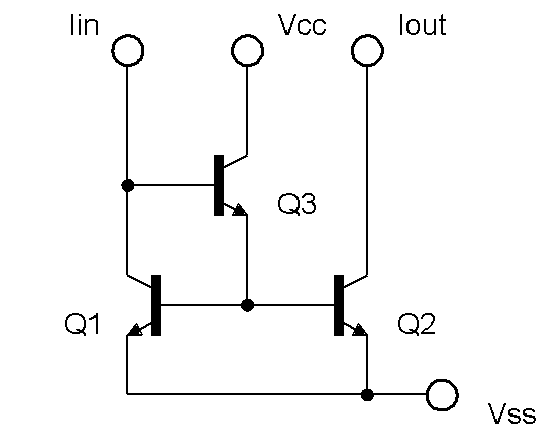
\includegraphics[scale=0.5]{obrazky/ZlepseneWilsonovoZrcadloNPN}
%  \end{center}
%  \caption[Alenčino zrcadlo]{Zlepšené Wilsonovo proudové zrcadlo.}
%\end{figure}
%
%Pro sazbu vektorových obrázků přímo v~\LaTeX{}u je možné doporučit balíček \href{https://www.ctan.org/pkg/pgf}{\texttt{TikZ}}.
%Příklady sazby je možné najít na \href{http://www.texample.net/tikz/examples/}{\TeX{}ample}.
%Pro vyzkoušení je možné použít programy QTikz nebo TikzEdt.
%
%
%
%
%\chapter{Příklad sazby zdrojových kódů}
%
%\section{Balíček \texttt{listings}}
%
%Pro vysázení zdrojových souborů je možné použít balíček \href{https://www.ctan.org/pkg/listings}{\texttt{listings}}.
%Balíček zavádí nové prostředí \texttt{lstlisting} pro sazbu zdrojových kódů, jako například:
%%
%\begin{lstlisting}[language={[LaTeX]TeX}]
%\section{Balíček lstlistings}
%Pro vysázení zdrojových souborů je možné použít
%	balíček \href{https://www.ctan.org/pkg/listings}%
%	{\texttt{listings}}.
%Balíček zavádí nové prostředí \texttt{lstlisting} pro
%	sazbu zdrojových kódů.
%\end{lstlisting}
%%
%Podporuje množství programovacích jazyků.
%Kód k~vysázení může být načítán přímo ze zdrojových souborů.
%Umožňuje vkládat čísla řádků nebo vypisovat jen vybrané úseky kódu.
%Např.:
%
%\noindent
%Zkratky jsou sázeny v~prostředí \texttt{acronym}:
%\label{lst:zkratky}
%\lstinputlisting[language={[LaTeX]TeX},nolol,numbers=left, firstnumber=6, firstline=6,lastline=6]{text/zkratky.tex}
%%
%Šířka textu volitelného parametru \verb|KolikMista| udává šířku prvního sloupce se zkratkami.
%Proto by měla být zadávána nejdelší zkratka nebo symbol.
%Příklad definice zkratky \acs{symfvz} je na výpisu \ref{lst:symfvz}.
%
%\shorthandoff{-}
%\lstinputlisting[language={[LaTeX]TeX},frame=single,caption={Ukázka sazby zkratek},label=lst:symfvz,numbers=left,linerange={bsymfvz-\%\%\%\ esymfvz},includerangemarker=false]{text/zkratky.tex}
%\shorthandon{-}
%
%\noindent
%Ukončení seznamu je provedeno ukončením prostředí:
%\lstinputlisting[language={[LaTeX]TeX},nolol,numbers=left,firstnumber=26,linerange=26]{text/zkratky.tex}
%
%\vspace{\fill}
%
%\noindent
%{\bf Poznámka k~výpisům s~použitím volby jazyka \verb|czech| nebo \verb|slovak|:}\newline
%Pokud Váš zdrojový kód obsahuje znak spojovníku \verb|-|, pak překlad může skončit chybou.
%Ta je způsobená tím, že znak \verb|-| je v~českém nebo slovenském nastavení balíčku \verb|babel| tzv.\ aktivním znakem.
%Přepněte znak \verb|-| na neaktivní příkazem \verb|\shorthandoff{-}| těsně před výpisem a hned za ním jej vraťte na aktivní příkazem \verb|\shorthandon{-}|.
%Podobně jako to je ukázáno ve zdrojovém kódu šablony.
%
%
%\clearpage
%
%%\section{Výpis kódu prostředí Matlab}
%Na výpisu \ref{lst:priklad.vypis.kodu.Matlab} naleznete příklad kódu pro Matlab, na výpisu \ref{lst:priklad.vypis.kodu.C} zase pro jazyk~C.
%
%\lstnewenvironment{matlab}[1][]{%
%\iflanguage{czech}{\shorthandoff{-}}{}%
%\iflanguage{slovak}{\shorthandoff{-}}{}%
%\lstset{language=Matlab,numbers=left,#1}%
%}{%
%\iflanguage{slovak}{\shorthandon{-}}{}%
%\iflanguage{czech}{\shorthandon{-}}{}%
%}
%
%\begin{matlab}[frame=single,float=htbp,caption={Příklad Schur-Cohnova testu stability v~prostředí Matlab.},label=lst:priklad.vypis.kodu.Matlab,numberstyle=\scriptsize, numbersep=7pt]
%%% Priklad testovani stability filtru
%
%% koeficienty polynomu ve jmenovateli
%a = [ 5, 11.2, 5.44, -0.384, -2.3552, -1.2288];
%disp( 'Polynom:'); disp(poly2str( a, 'z'))
%
%disp('Kontrola pomoci korenu polynomu:');
%zx = roots( a);
%if( all( abs( zx) < 1))
%    disp('System je stabilni')
%else
%    disp('System je nestabilni nebo na mezi stability');
%end
%
%disp(' '); disp('Kontrola pomoci Schur-Cohn:');
%ma = zeros( length(a)-1,length(a));
%ma(1,:) = a/a(1);
%for( k = 1:length(a)-2)
%    aa = ma(k,1:end-k+1);
%    bb = fliplr( aa);
%    ma(k+1,1:end-k+1) = (aa-aa(end)*bb)/(1-aa(end)^2);
%end
%
%if( all( abs( diag( ma.'))))
%    disp('System je stabilni')
%else
%    disp('System je nestabilni nebo na mezi stability');
%end
%\end{matlab}
%
%\noindent
%\begin{minipage}{\linewidth}
%
%
%%\section{Výpis kódu jazyka C}
%
%\begin{lstlisting}[frame=single,numbers=right,caption={Příklad implementace první kanonické formy v~jazyce C.},label=lst:priklad.vypis.kodu.C,basicstyle=\ttfamily\small, keywordstyle=\color{black}\bfseries\underbar,]
%// první kanonická forma
%short fxdf2t( short coef[][5], short sample)
%{
%	static int v1[SECTIONS] = {0,0},v2[SECTIONS] = {0,0};
%	int x, y, accu;
%	short k;
%
%	x = sample;
%	for( k = 0; k < SECTIONS; k++){
%		accu = v1[k] >> 1;
%		y = _sadd( accu, _smpy( coef[k][0], x));
%		y = _sshl(y, 1) >> 16;
%
%		accu = v2[k] >> 1;
%		accu = _sadd( accu, _smpy( coef[k][1], x));
%		accu = _sadd( accu, _smpy( coef[k][2], y));
%		v1[k] = _sshl( accu, 1);
%
%		accu = _smpy( coef[k][3], x);
%		accu = _sadd( accu, _smpy( coef[k][4], y));
%		v2[k] = _sshl( accu, 1);
%
%		x = y;
%	}
%	return( y);
%}
%\end{lstlisting}
%\end{minipage}
%
%
%
%
%
%
%
%\chapter{Obsah elektronické přílohy}
%Elektronická příloha je často nedílnou součástí semestrální nebo závěrečné práce.
%Vkládá se do informačního systému VUT v~Brně ve vhodném formátu (ZIP, PDF\,\dots).
%
%Nezapomeňte uvést, co čtenář v~této příloze najde.
%Je vhodné okomentovat obsah každého adresáře, specifikovat, který soubor obsahuje důležitá nastavení, který soubor je určen ke spuštění, uvést nastavení kompilátoru atd.
%Také je dobře napsat, v~jaké verzi software byl kód testován (např.\ Matlab 2018b).
%Pokud bylo cílem práce vytvořit hardwarové zařízení,
%musí elektronická příloha obsahovat veškeré podklady pro výrobu (např.\ soubory s~návrhem DPS v~Eagle).
%
%Pokud je souborů hodně a jsou organizovány ve více složkách, je možné pro výpis adresářové struktury použít balíček \href{https://www.ctan.org/pkg/dirtree}{\texttt{dirtree}}.
%
%\bigskip
%
\chapter{Contents of the Enclosed Electronic Appendix}
\label{ch:flash_contents}
{\small
%
\dirtree{%.
.1 /\DTcomment{Root}.
.2 .github\DTcomment{CI workflows and auxiliary files}.
.2 Hardware\DTcomment{Hardware resources for both HW revisions}.
.3 Cube\DTcomment{STM32CubeMX project for pin assigment}.
.3 Docs\DTcomment{Datasheets of components}.
.3 Libs\DTcomment{KiCAD component and footprint libraries}.
.3 rev1\DTcomment{KiCAD project for the first revision}.
.3 rev2\DTcomment{KiCAD project for the second revision}.
.2 Poster\DTcomment{Source file for a future poster}.
.3 poster\_template.pptx.
.2 Software\DTcomment{Software projects and source code}.
.3 controller\DTcomment{The control software}.
.3 embedded\DTcomment{Workspace containing cross-compiled projects}.
.4 firmware\DTcomment{The motor controller's firmware}.
.4 testsuite\DTcomment{Tests for the motor controller's firmware}.
.3 shared\DTcomment{Project with code shared between firmware and controller}.
.3 Cargo.toml\DTcomment{Cargo project file}.
.3 Cargo.lock\DTcomment{Cargo project file lock}.
.3 LICENSE-MIT\DTcomment{Software License}.
.3 README.md\DTcomment{Read me for software}.
.2 Thesis\DTcomment{Source code for this thesis}.
.2 README.md\DTcomment{Readme for this master's project}.
}
}

\chapter{Schematic of the Second Electronics Revision}
\label{ch:rev2_schematic}
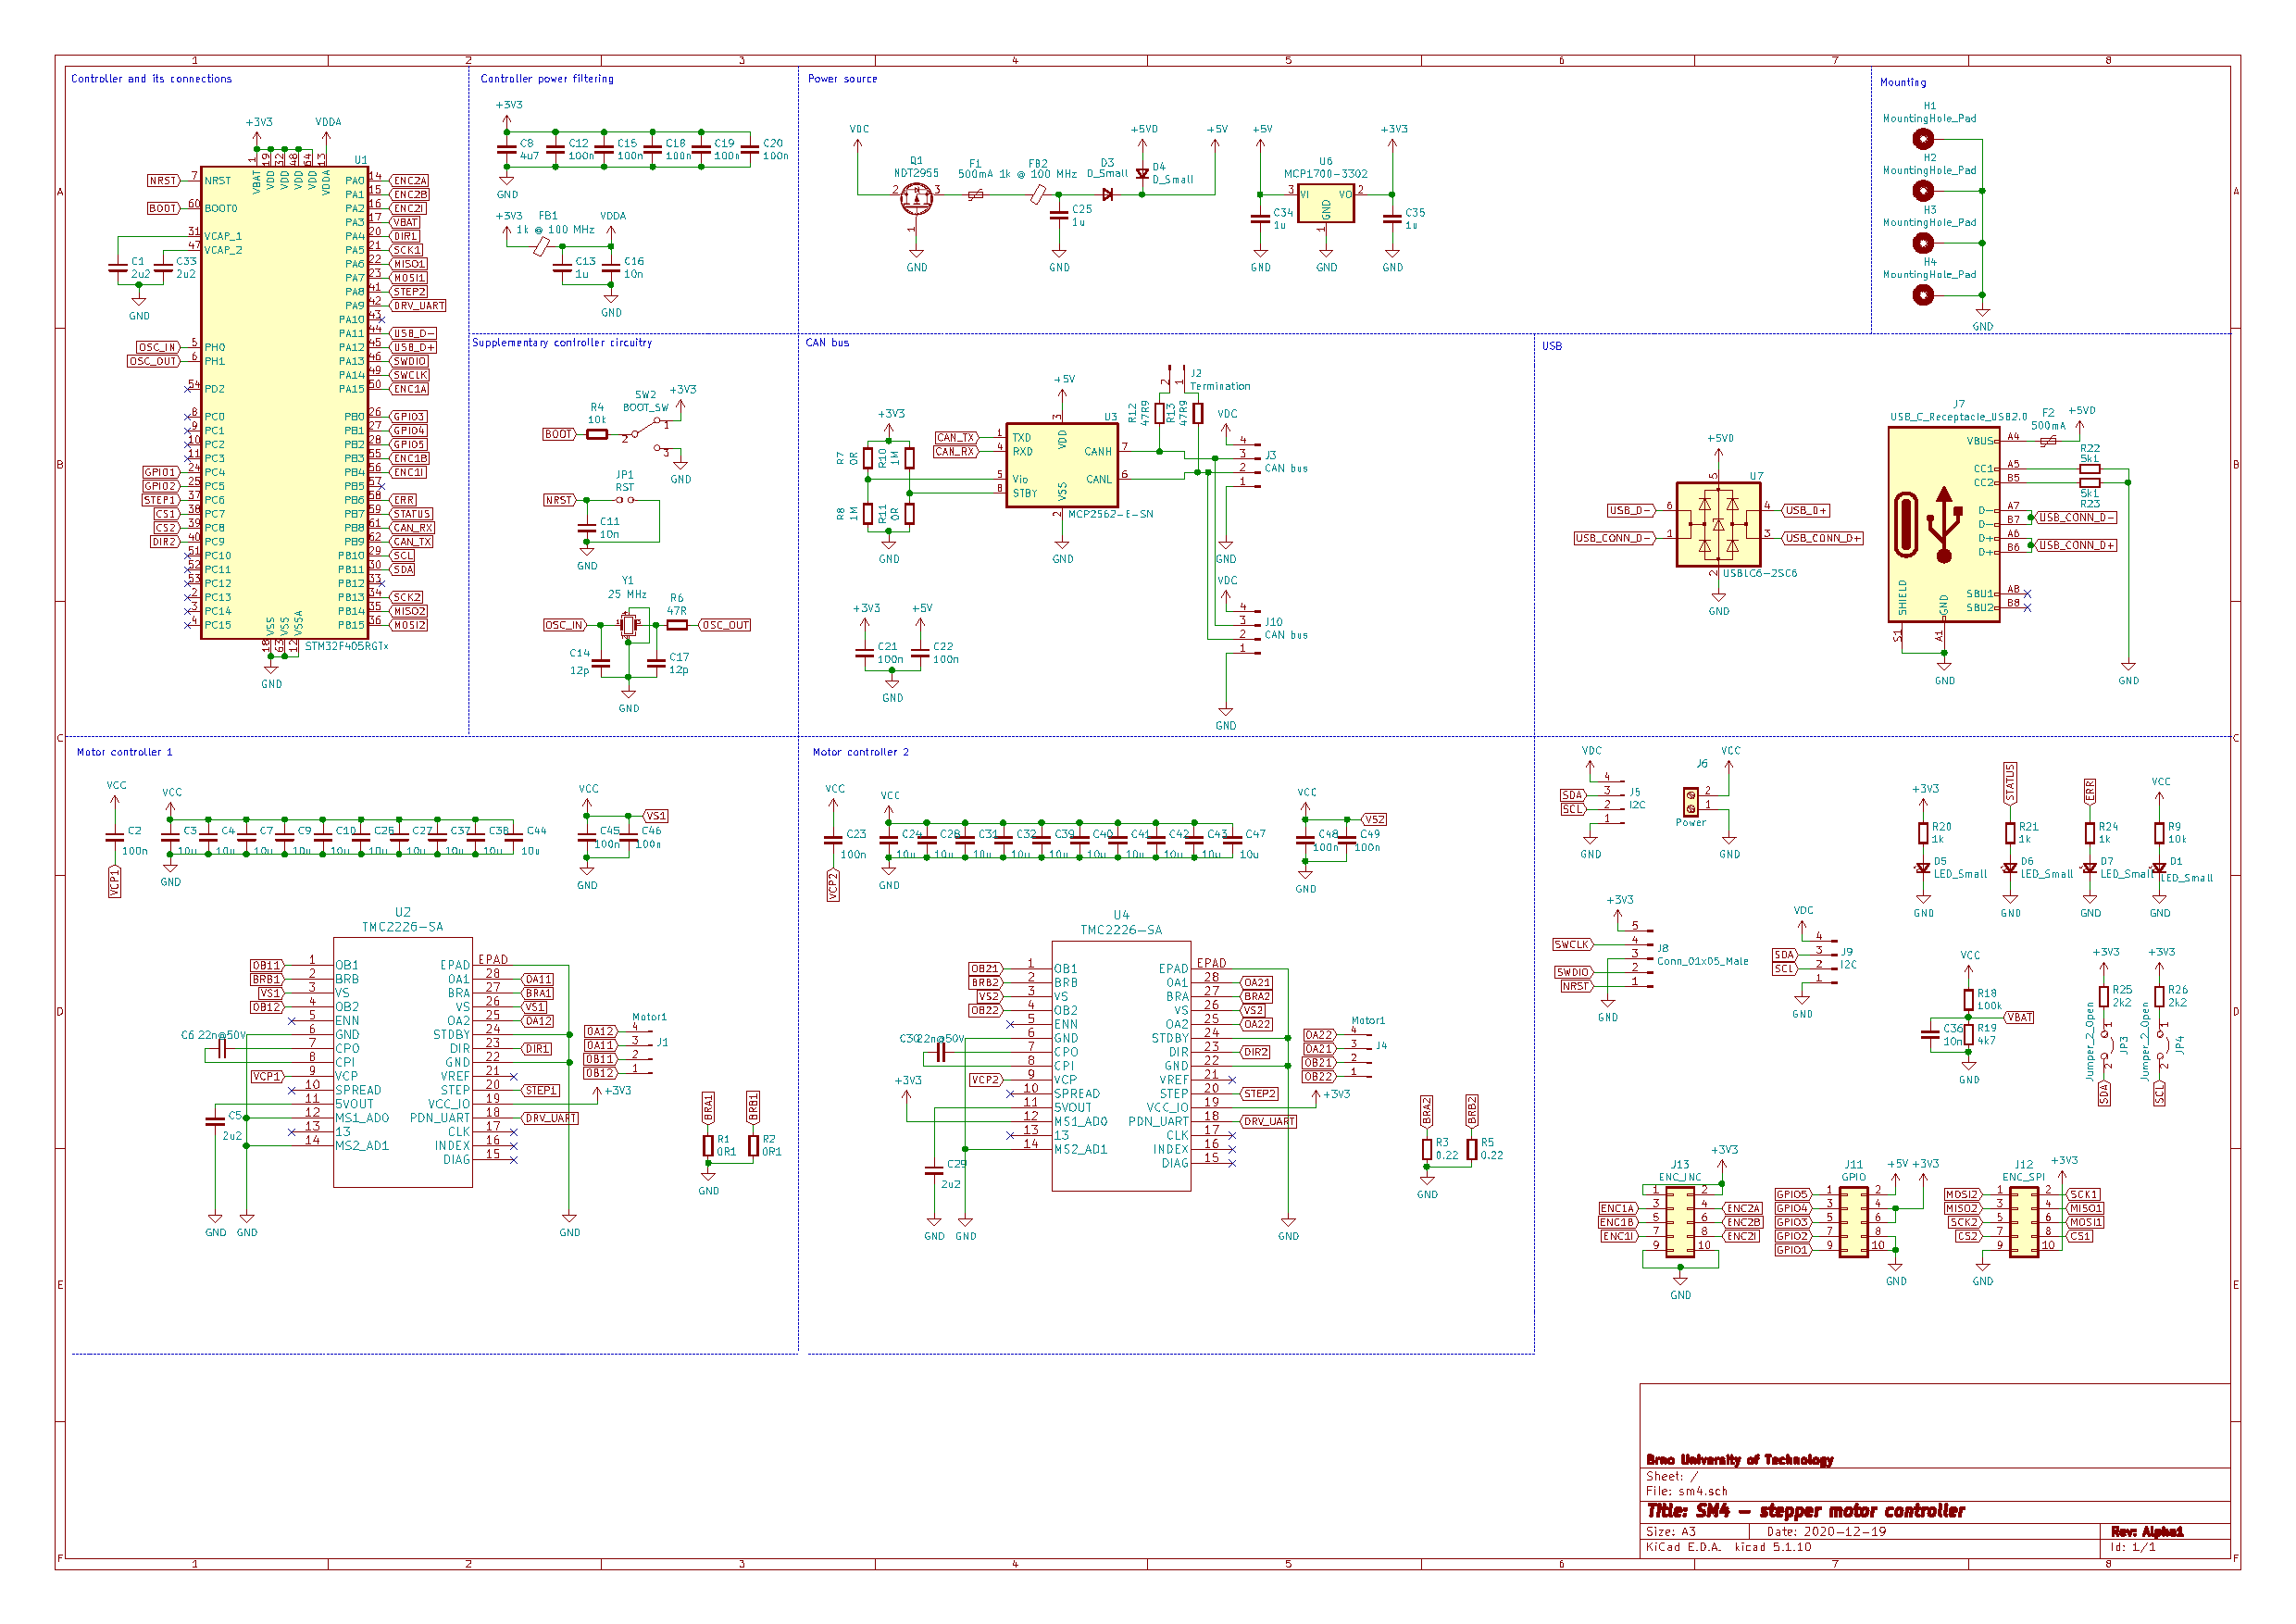
\includepdf[pages=1, landscape=true]{pdf/schematic}

\chapter{PCB of the Second Electronics Revision}
\label{ch:rev2_pcb}
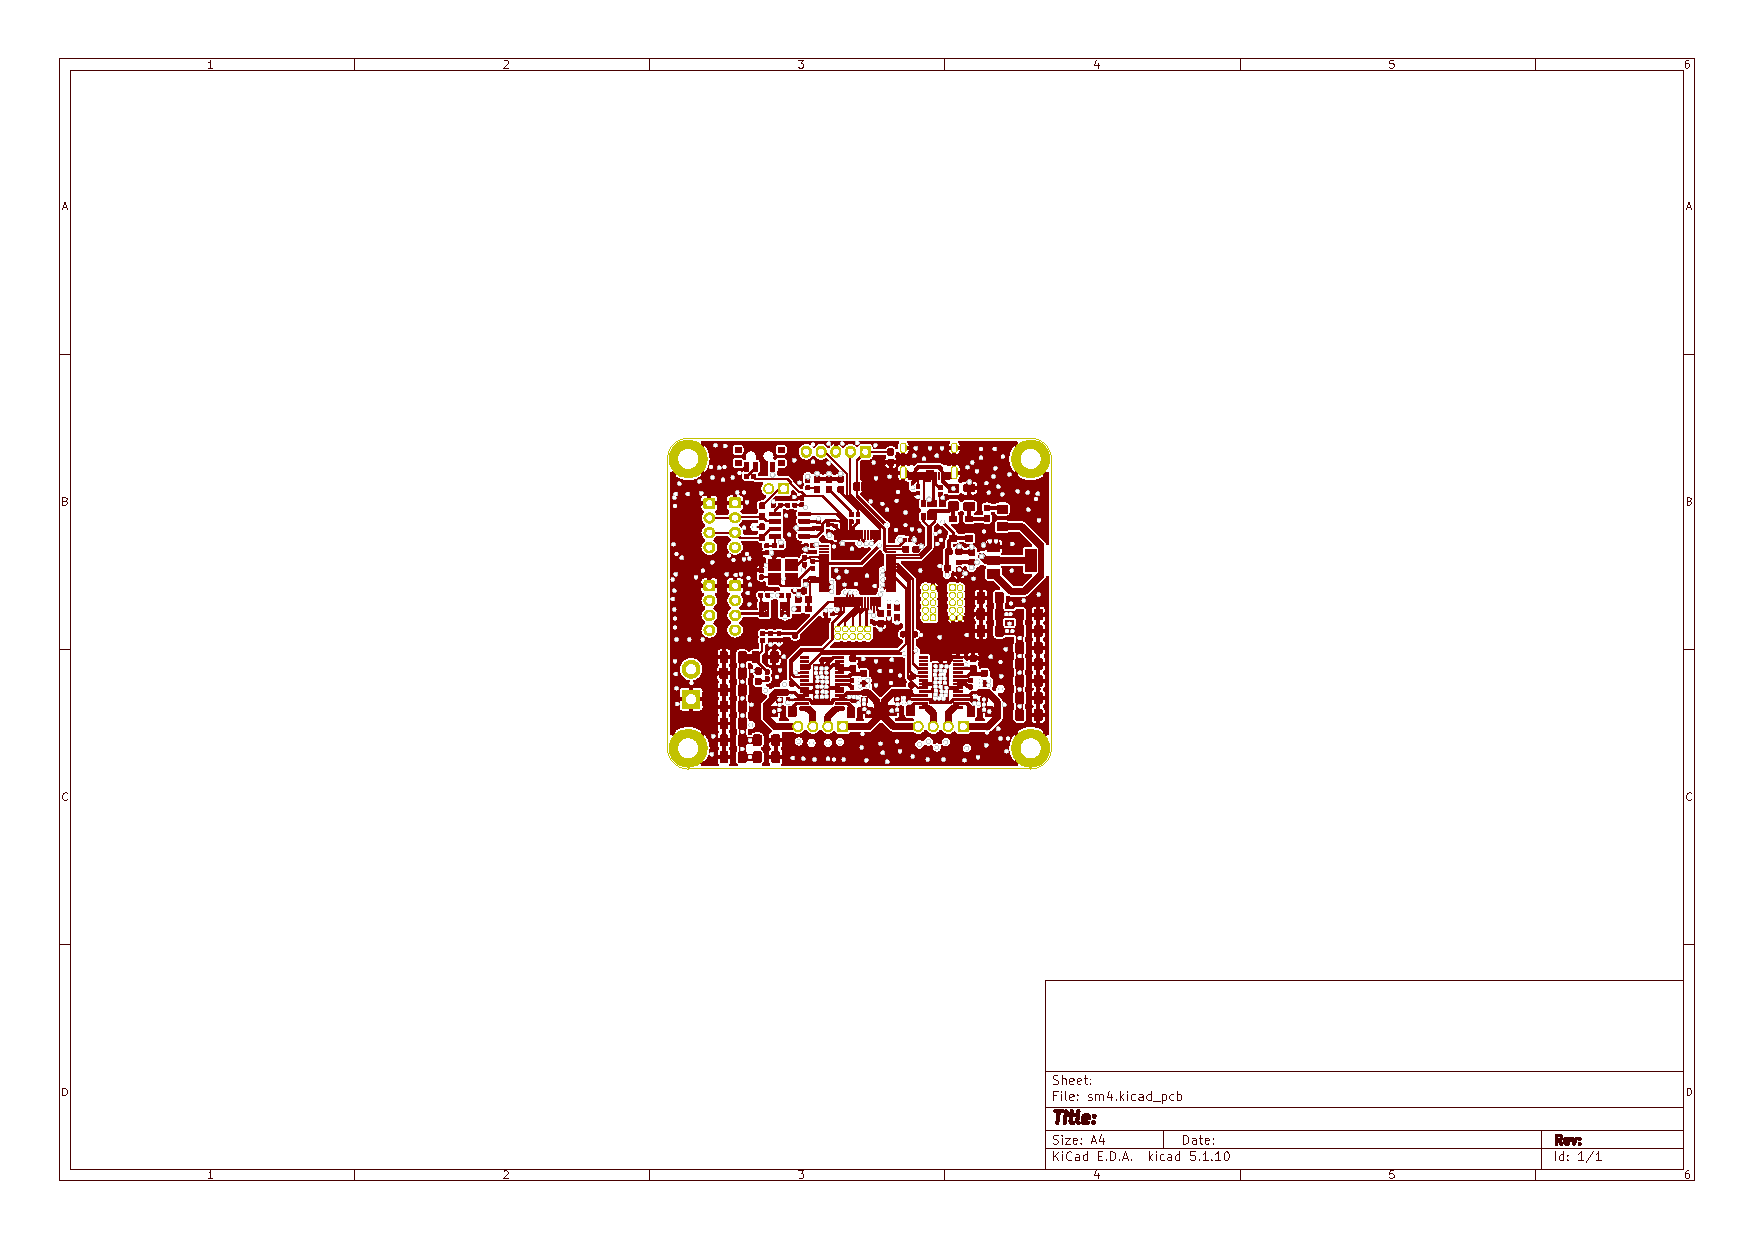
\includepdf[pages=-, landscape=true]{pdf/pcb}

\chapter{CANOpen PDOs and Object Dictionary}
\label{ch:canopen_appendices}
\begin{table}[H]
    \centering
    \begin{tabular}{ |p{1.5cm}|p{1.8cm}|p{1.8cm}|p{2cm}|p{5.5cm}| }
        \hline
        Index & Subindex & Type & Length [B] & Description \\
        \hline
        \hline
        2000 & 1 & f32 & 4 & Battery Voltage in Volts \\
        \hline
        2000 & 2 & f32 & 4 & MCU Temperature in \textdegree C \\
        \hline
        2[1,2]00 & 1 & AxisMode & 1 & mode of the axis - 0 for velocity, 1 for position \\
        \hline
        2[1,2]00 & 2 & bool & 1 & axis enabled \\
        \hline
        2[1,2]00 & 3 & f32 & 4 & target axis velocity in RPS \\
        \hline
        2[1,2]00 & 4 & f32 & 4 & actual axis velocity in RPS \\
        \hline
        2[1,2]00 & 5 & i32 & 4 & target axis position - revolutions \\
        \hline
        2[1,2]00 & 6 & u32 & 4 & target axis position - angle \\
        \hline
        2[1,2]00 & 7 & i32 & 4 & actual axis position - revolutions \\
        \hline
        2[1,2]00 & 8 & u32 & 4 & actual axis position - angle \\
        \hline
        2[1,2]00 & 9 & f32 & 4 & target ramp acceleration in RPS per second \\
        \hline
        2[1,2]00 & 10 & bool & 1 & velocity controller bypass enabled \\
        \hline
        2[1,2]00 & 11 & f32 & 4 & current applied to motor winding during acceleration in Amperes \\
        \hline
        2[1,2]00 & 12 & f32 & 4 & current applied to motor winding when idle in Amperes \\
        \hline
        2[1,2]00 & 13 & f32 & 4 & current applied to motor winding when moving with constant speed in Amperes \\
        \hline
        2[1,2]00 & 14 & f32 & 4 & velocity controller proportional gain \\
        \hline
        2[1,2]00 & 15 & f32 & 4 & velocity controller summation gain \\
        \hline
        2[1,2]00 & 16 & f32 & 4 & velocity controller differential gain \\
        \hline
        2[1,2]00 & 17 & f32 & 4 & velocity controller maximal action value \\
        \hline
        2[1,2]00 & 18 & f32 & 4 & position controller proportional gain \\
        \hline
        2[1,2]00 & 19 & f32 & 4 & position controller summation gain \\
        \hline
        2[1,2]00 & 20 & f32 & 4 & position controller differential gain \\
        \hline
        2[1,2]00 & 21 & f32 & 4 & position controller maximal action value \\
        \hline
    \end{tabular}
    \caption{RxPDO1 mapping}
    \label{tab:object_dictionary}
\end{table}

\begin{table}[H]
    \centering
    \begin{tabular}{ |p{3cm}|p{2cm}|p{8cm}| }
        \hline
        Value & Length [B] & Description \\
        \hline
        \hline
        axis mode & 1 & LSB contains axis 1 mode - 0 means velocity mode, 1 means position mode, first bit of the second nimble contains axis 2 mode \\
        \hline
        axis enabled & 1 & LSB sets axis 1 enabled - 0 means disabled, 1 means enabled, second lowest bit sets axis 2 enabled \\
        \hline
    \end{tabular}
    \caption{RxPDO1 mapping}
    \label{tab:rxpdo1}
\end{table}

\begin{table}[H]
    \centering
    \begin{tabular}{ |p{3cm}|p{2cm}|p{8cm}| }
        \hline
        Value & Length [B] & Description \\
        \hline
        \hline
        battery voltage & 2 & battery voltage in millivolts \\
        \hline
        temperature & 2 & temperature in tenths of \textdegree C \\
        \hline
    \end{tabular}
    \caption{TxPDO1 mapping}
    \label{tab:txpdo1}
\end{table}


RxPDO2, TxPDO2
\begin{table}[H]
    \centering
    \begin{tabular}{ |p{3cm}|p{2cm}|p{8cm}| }
        \hline
        Value & Length [B] & Description \\
        \hline
        \hline
        axis 1 velocity & 4 & 32-bit float indicating axis 1 velocity in revolutions per second \\
        \hline
        axis 2 velocity & 4 & 32-bit float indicating axis 2 velocity in revolutions per second \\
        \hline
    \end{tabular}
    \caption{Mapping of PDOs containing velocity information - RxPDO2 and TxPDO2}
    \label{tab:velocity_pdo}
\end{table}

\begin{table}[H]
    \centering
    \begin{tabular}{ |p{3cm}|p{2cm}|p{8cm}| }
        \hline
        Value & Length [B] & Description \\
        \hline
        \hline
        axis revolutions & 4 & signed 32-bit integer denoting the number of axis shaft revolutions \\
        \hline
        axis angle & 4 & unsigned 32-bit indicating axis shaft angle \\
        \hline
    \end{tabular}
    \caption{Mapping of PDOs containing position information - RxPDO3, RxPDO4, TxPDO3 and TxPDO4}
    \label{tab:position_pdo}
\end{table}



\end{document}